\documentclass[12pt, a4paper, oneside]{report}

% Font and Encoding
\usepackage[utf8]{inputenc}
\usepackage{mathptmx} % Times New Roman roughly equivalent
\usepackage[T1]{fontenc}

% Margins setup
% Left 1.5 inches except the Front Cover (1.2 inches), Right 1 inch, Top/Bottom 1 inch.
% Header/Footer 0.5/0.4 inch.
\usepackage[left=1.5in, right=1in, top=1in, bottom=1in, headheight=15pt, headsep=0.25in, footskip=0.6in]{geometry}

% Line Spacing (1.5)
\usepackage{setspace}
\onehalfspacing

% Headers and Footers
\usepackage{fancyhdr}
\pagestyle{fancy}
\fancyhf{} % Clear all header and footer fields
% Header Align left: chapter number and title
\renewcommand{\chaptermark}[1]{\markboth{\thechapter\ #1}{}}
\lhead{\leftmark}
% Footer Align left: Dept info. Align right: Page Number
\lfoot{\footnotesize BTech CSE (CSE/IT/CSN/AI) \\ School of Computer Science Engineering \& Technology}
\rfoot{\thepage}
\renewcommand{\headrulewidth}{0.4pt}
\renewcommand{\footrulewidth}{0.4pt}

% Styling for chapters and sections (Times New Roman 12pt black)
\usepackage{titlesec}
\titleformat{\chapter}[display]
  {\normalfont\bfseries\centering}{\chaptertitlename\ \thechapter}{12pt}{\Large}
\titleformat{\section}
  {\normalfont\bfseries}{\thesection}{1em}{}
\titleformat{\subsection}
  {\normalfont\bfseries}{\thesubsection}{1em}{}

% Bibliography (Harvard Style)
\usepackage[authoryear, round]{natbib}

% Graphics and other utilities
\usepackage{graphicx}
\usepackage{hyperref}
\usepackage{cleveref}
\usepackage{tikz}
\usetikzlibrary{shapes.geometric, arrows.meta, positioning, calc}
\usepackage{pgfplots}
\pgfplotsset{compat=1.18}
\usepackage{booktabs}
\usepackage{tabularx}
\usepackage{longtable}
\usepackage{caption}
\usepackage{listings}
\usepackage{xcolor}

\lstset{
    basicstyle=\ttfamily\small,
    breaklines=true,
    breakatwhitespace=true,
    postbreak=\mbox{\textcolor{red}{$\hookrightarrow$}\space},
    columns=fullflexible,
    keepspaces=true,
    frame=single,
    xleftmargin=0pt,
    xrightmargin=0pt
}


% Exception for Table/Figure font sizes (10 to 11 pt)
\captionsetup{font=small} % 11pt approx when main font is 12pt

\begin{document}

% Overriding margin for Front Cover (1.2 inches left instead of 1.5)
\newgeometry{left=1.2in, right=1in, top=1in, bottom=1in}
\begin{titlepage}
    \centering
    \vspace*{2cm}
    
    {\fontsize{14pt}{16.8pt}\selectfont \textbf{Design and Implementation of HomeSOC:\\ A Lightweight Local Security Operations Center}\par}
    
    \vspace{3cm}
    
    {\fontsize{12pt}{14.4pt}\selectfont \textbf{A Project Thesis submitted in partial fulfillment of the requirements for the degree of}\par}
    
    \vspace{1cm}
    {\fontsize{12pt}{14.4pt}\selectfont \textbf{Bachelor of Technology (BTech)}\par}
    {\fontsize{12pt}{14.4pt}\selectfont \textbf{in}\par}
    {\fontsize{12pt}{14.4pt}\selectfont \textbf{Computer Science and Engineering}\par}
    
    \vspace{2cm}
    
    {\fontsize{12pt}{14.4pt}\selectfont \textbf{By}\par}
    \vspace{0.5cm}
    {\fontsize{12pt}{14.4pt}\selectfont \textbf{[Your Name] \hspace{1cm} [Enrollment Number]}\par}
    
    \vfill
    
    % Note: Logo omitted as per instructions
    {\fontsize{12pt}{14.4pt}\selectfont \textbf{School of Computer Science Engineering \& Technology}\par}
    {\fontsize{12pt}{14.4pt}\selectfont \textbf{[University Name]}\par}
    {\fontsize{12pt}{14.4pt}\selectfont \textbf{2026}\par}
\end{titlepage}
\restoregeometry % Revert to 1.5in left margin after cover

% Start Roman numbering for Front Matter
\pagenumbering{roman}
\setcounter{page}{1}

% Report Status Declaration Form
\chapter*{Report Status Declaration Form}
\addcontentsline{toc}{chapter}{Report Status Declaration Form}
\vspace{1cm}
I hereby declare that this thesis is my original work and has not been submitted to any other university or institution for any degree. The research presented here was conducted in accordance with the university guidelines.
\vspace{2cm}\\
\noindent
Author Signature: \rule{5cm}{1pt} \\
Date: \rule{3cm}{1pt} \\

\clearpage

% Secondary Title Page
\chapter*{Title Page}
\addcontentsline{toc}{chapter}{Title Page}
\begin{center}
    \vspace*{2cm}
    {\fontsize{14pt}{16.8pt}\selectfont \textbf{Design and Implementation of HomeSOC:\\ A Lightweight Local Security Operations Center}\par}
    \vspace{2cm}
    {\fontsize{12pt}{14.4pt}\selectfont \textbf{By}\par}
    {\fontsize{12pt}{14.4pt}\selectfont \textbf{[Your Name]}\par}
    \vspace{2cm}
    {\fontsize{12pt}{14.4pt}\selectfont \textbf{Under the supervision of}\par}
    {\fontsize{12pt}{14.4pt}\selectfont \textbf{[Supervisor Name]}\par}
\end{center}

\clearpage

% Declaration of Originality
\chapter*{Declaration of Originality}
\addcontentsline{toc}{chapter}{Declaration of Originality}
This is to certify that the project report entitled ``Design and Implementation of HomeSOC: A Lightweight Local Security Operations Center'' submitted by [Your Name], Enrollment Number [Enrollment], for the award of Bachelor of Technology (BTech) in Computer Science and Engineering from the School of Computer Science Engineering \& Technology, is a bonafide record of original research work carried out under my supervision. The contents of this report, in full or in parts, have not been submitted to any other Institution or University for the award of any degree or diploma.
\vspace{2cm}\\
\noindent
\rule{5cm}{1pt} \\
\textbf{Supervisor Name}\\

\clearpage

% Acknowledgements
\chapter*{Acknowledgements}
\addcontentsline{toc}{chapter}{Acknowledgements}
Sincere gratitude is extended to all individuals who provided guidance and support during the development of this project. Special appreciation is given to the project supervisor for their invaluable insights, continuous encouragement, and technical feedback throughout the research and implementation phases. Furthermore, gratitude is expressed to the faculty members of the School of Computer Science Engineering \& Technology for establishing a foundation of knowledge that made this complex security engineering project possible. 

\clearpage

% Abstract
\chapter*{Abstract}
\addcontentsline{toc}{chapter}{Abstract}
With the proliferation of connected devices in home and small office networks, managing local security threats has become increasingly complex. While large-scale enterprises rely on sophisticated Security Information and Event Management (SIEM) systems and Security Operations Centers (SOC), these solutions are fundamentally too resource-intensive, expensive, and opaque for residential or lightweight deployments. This thesis presents the design, methodology, and implementation of ``HomeSOC'', a highly efficient, lightweight local Security Operations Center explicitly architected for small-scale networks. 

The primary problem addressed was the lack of an accessible, low-latency alerting system capable of monitoring local hosts without deploying enterprise-grade infrastructure. The proposed approach developed a Python-based host agent script tailored for local telemetry collection (including authentication logs, process state, and system metrics) alongside a robust detection engine driven by a centralised Flask server. To handle concurrent data ingestion and ensure data integrity under high volume, SQLite was leveraged with Write-Ahead Logging (WAL) concurrency controls. The entire system was transitioned from a local prototype to a fully containerised cloud deployment hosted on PythonAnywhere. 

The research process validated the capability of HomeSOC to instantly detect, categorise, and triage anomalies like brute-force attacks, suspected cryptominers, and spear-phishing attempts. Through the development of an intelligent, dynamic web dashboard featuring zero-latency asynchronous Javascript polling and custom threshold alerts, the project achieved a sophisticated, aesthetically premium monitoring solution. The conclusion confirms that a robust security framework can be attained on lightweight hardware, offering novel contributions to affordable network visibility, and paving the pathway for machine-learning-driven predictive anomaly detection in future iterations.

\clearpage

% Table of Contents
\tableofcontents
\clearpage

% List of Tables
\listoftables
\addcontentsline{toc}{chapter}{List of Tables}
\clearpage

% List of Figures
\listoffigures
\addcontentsline{toc}{chapter}{List of Figures}
\clearpage

% List of Symbols
\chapter*{List of Symbols}
\addcontentsline{toc}{chapter}{List of Symbols}
\begin{tabular}{ll}
\% & Percentage (used in CPU and Memory load metrics) \\
/ & Directory path separator \\
$>$ & Greater than (used in logical alert triggers) \\
$<$ & Less than \\
\end{tabular}

\clearpage

% List of Abbreviations
\chapter*{List of Abbreviations}
\addcontentsline{toc}{chapter}{List of Abbreviations}
\begin{tabular}{ll}
API & Application Programming Interface \\
CPU & Central Processing Unit \\
CSS & Cascading Style Sheets \\
HTML & HyperText Markup Language \\
JSON & JavaScript Object Notation \\
MVP & Minimum Viable Product \\
OS & Operating System \\
RAM & Random Access Memory \\
SIEM & Security Information and Event Management \\
SOC & Security Operations Center \\
SQL & Structured Query Language \\
UI & User Interface \\
WAL & Write-Ahead Logging \\
\end{tabular}

\clearpage


% Start Arabic numbering for Chapters
\clearpage
\pagenumbering{arabic}
\setcounter{page}{1}

\chapter{Introduction}

\section{Background of Cybersecurity Monitoring}
The exponential expansion of digital infrastructure over the past three decades has fundamentally revolutionized global communication, commerce, and personal connectivity. However, this architectural metamorphosis has been closely mirrored by a massive, corresponding escalation in malicious cyber activity. In the nascent stages of network computing, the perimeter was distinctly defined: a physical local area network (LAN) isolated geographically within a corporate office, guarded by a singular hardware firewall appliance. Modern topography, however, has effectively dissolved this concept. The pervasive integration of cloud computing architectures, ubiquitous mobile connectivity, and the aggressive proliferation of the Internet of Things (IoT) have catalyzed a ubiquitous, borderless digital environment. 

This boundless connectivity, whilst technologically liberating, has exponentially expanded the accessible attack surface available to threat actors. Devices that were historically sequestered behind robust enterprise security perimeters are now constantly exposed natively to the public internet. Consequently, network administrators and security engineers are no longer tasked simply with repelling external attacks against a hardened gateway; they must continually monitor, analyze, and audit internal network lateral movement, anomalous process executions, and cryptic authentication failures occurring simultaneously across thousands of heterogeneous, independent host nodes.

To mitigate this complex threat landscape, the Information Security (InfoSec) industry conceived and deployed specialized analytical frameworks designed to ingest and parse massive volumes of operational telemetry. This evolutionary process crystallized in the formulation of the Security Operations Center (SOC) paradigm and its core technological mechanism: the Security Information and Event Management (SIEM) system.

\section{The Evolution of Network Threats}
Understanding the necessity of a localized monitoring solution necessitates a precise analysis of modern threat capabilities, distinctly regarding the shift from highly targeted corporate espionage vectors toward indiscriminate, automated payload delivery campaigns.

For decades, Advanced Persistent Threats (APTs) driven by nation-state actors focused exclusively on compromising high-value corporate intellectual property or critical sovereign infrastructure. The substantial cost, time, and specialized knowledge required to breach these fortified perimeters meant that small-to-medium enterprises (SMEs) and residential networks were largely perceived as statistically insignificant targets, lacking sufficient financial reward to justify the deployment of complex zero-day exploit arsenals.

However, the advent of cryptocurrency integration, coupled inextricably with the commoditization of malicious software through decentralized "Malware-as-a-Service" (MaaS) distribution frameworks, fundamentally disrupted this calculus. Cybercriminal syndicates pivoted aggressively toward indiscriminate, automated scanning arrays exploiting low-hanging vulnerabilities universally across the global IPv4 spectrum. 

\subsection{The Internet of Things (IoT) Vulnerability Vector}
A primary catalyst driving this shift is the deployment of IoT appliances within unmonitored home networks. The typical modern residential environment or small office inherently hosts a volatile, heterogeneous blend of consumer-grade technologies:
\begin{itemize}
    \item Smart television sets operating unpatched, proprietary Linux kernels.
    \item Network-Attached Storage (NAS) drives containing unencrypted personal data exposed directly to remote subnets via incorrect port-forwarding configurations.
    \item Intelligent thermostats, smart speakers, and automated lighting systems relying entirely on deprecated cryptographic libraries (e.g., outdated TLS/SSL protocols).
    \item Mobile phones and legacy laptops routinely bypassing security protocols by connecting periodically to unsecured public Wi-Fi access points before returning to the trusted internal subnet.
\end{itemize}

These devices represent an incredibly asymmetric vulnerability. Manufacturers frequently fail to issue proactive firmware patching updates, relying extensively on static, hardcoded default administrative passwords (e.g., `admin/admin` or `root/toor`). Consequently, these innocuous appliances present a completely frictionless entry point for automated botnets (most notably exemplified by the Mirai malware architecture) seeking to hijack computational resources.

\subsection{Adversary Objectives in Local Environments}
Once an initial foothold is established within a previously trusted, unmonitored local network, the adversary's operational objectives are rarely restricted to the initially compromised endpoint. Modern attack campaigns execute distinct post-exploitation methodologies:
\begin{enumerate}
    \item \textbf{Lateral Reconnaissance}: The compromised terminal acts seamlessly as a covert internal pivot node, launching unrestricted ICMP sweeps and TCP SYN mapping arrays across the active subnet (typically via `Nmap`) to identify valuable active adjacent machines executing open RPC, RDP, or SMB protocols.
    \item \textbf{Clandestine Cryptojacking}: Instead of executing immediately disruptive ransomware logic, sophisticated actors silently deploy obfuscated CPU-intensive cryptocurrency mining binaries (such as `XMRig`). These binaries algorithmically hijack the local hardware processor clocks, perpetually generating financial revenue for the adversary at the direct expense of the victim's electrical utility consumption and hardware longevity.
    \item \textbf{Data Exfiltration}: Aggressive indexing scripts covertly search user directories, harvesting financial credentials, session cookies, password databases, and cryptographic SSH keys prior to transmitting the compressed payload via encrypted DNS tunnels or standard HTTPS port 443 routes outwardly to Command and Control (C2) servers.
    \item \textbf{Extortion via Ransomware}: Executing a coordinated cryptographic locking mechanism universally encrypting connected mapped network block drives and demanding digital currency remittance in exchange for the complex private decryption keys.
\end{enumerate}

\section{The Systemic Failure of Enterprise Solutions for SMEs}
Despite this violently escalating threat landscape ravaging smaller networks, the orthodox methodologies dictating network security monitoring remain severely misaligned, fundamentally over-engineered, and utterly out of reach for non-corporate consumers. 

The premier cybersecurity industry effectively relies entirely on enterprise-grade SIEM deployments. These highly sophisticated systems (architected by vendors such as Splunk, IBM, or LogRhythm) are meticulously engineered to aggregate petabytes of raw system event logs across global decentralized topologies. While structurally magnificent, embedding these environments within a residential home-lab or small business infrastructure presents three insurmountable barriers:

\begin{enumerate}
    \item \textbf{Prohibitive Financial Licensing}: Commercial SIEM vendors calculate subscription licensing models explicitly based upon the daily volumetric ingestion of raw Gigabytes (GB/day). Even a modest deployment generating minor internal telemetry logs quickly exceeds tens of thousands of dollars in annual recurring operational expenditure (OpEx).
    \item \textbf{Exorbitant Dedicated Hardware Prerequisites}: Implementing open-source alternatives, notably the ELK Stack (Elasticsearch, Logstash, Kibana) or Wazuh, bypasses commercial software licensing but intrinsically mandates the deployment of immense distributed computational hardware. Running a Java Virtual Machine (JVM) Elasticsearch cluster necessitates complex multi-node server configurations requiring minimums of 8GB to 16GB of dedicated random access memory (RAM) allocation per server node simply to avoid critical indexing crashes. This parameter utterly invalidates deployment upon legacy desktop hardware or cost-effective ARM-based minicomputers (e.g., Raspberry Pi).
    \item \textbf{Astronomical Configuration Complexity}: The intrinsic difficulty associated with mapping chaotic, unstructured log files into cleanly indexed JSON objects requires massive proficiency with Regular Expressions (REGEX), Grok filtering logic, and complex indexing parameters. Furthermore, enterprise platforms rarely supply "out-of-the-box" anomaly identification tailored to basic individual endpoint nodes; they actively command dedicated, highly trained security analysts manually hunting through the syntax databases to interpret the data effectively.
\end{enumerate}

Consequently, the vast statistical majority of local networks operate entirely blind. They execute locally without a functional, accessible, low-latency alerting system capable of transparently tracking active endpoints and formulating clear, actionable, real-time threat intelligence.

\section{Problem Statement}
Given the severe disconnect between the complex magnitude of modern automated cyber threats ravaging lower-tier network environments and the exorbitant, inaccessible parameters natively defining standard enterprise SOC deployments, an undeniable critical gap inherently exists within the cybersecurity engineering market. 

There is a distinct, measurable necessity for the research, design, and deployment of an intelligent, lightweight, deeply integrated local monitoring mechanism capable of replicating the core operational visibility principles of a SIEM framework without inheriting the staggering computational overhead, extreme deployment complexity, or prohibitive financial demands associated with standard industry models. The system must effectively detect, analyze, and communicate complex behavioral anomalies to non-expert users rapidly in real-time, relying exclusively upon minimal hardware dependencies and standard standard programmatic protocols.

\section{Background Motivation}
The fundamental motivation explicitly driving this research thesis natively extends significantly beyond mere academic programmatic pursuit; it is fundamentally rooted in the absolute democratization of cybersecurity visibility. 

Traditionally, network administrators attempting to secure individual host machines deploy heavy Endpoint Detection and Response (EDR) agents (e.g., CrowdStrike or SentinelOne). These proprietary agents constantly record native kernel operating behaviors, continually transmitting immense volumes of internal telemetry back to a centralized algorithm hosted exclusively by external third-party security vendors. While demonstrably effective, the underlying computational overhead required by these scanning agents on older, deprecated, or severely resource-constrained domestic hardware can initiate catastrophic degradation in system continuity. 

Moreover, severe data privacy concerns inherently materialize when local personal behavioral data—extending far beyond explicit security metrics into private web navigation histories, application execution tracking, and file integrity scanning—is completely permanently outsourced, evaluated, and perpetually archived by external corporations entirely outside the user's localized physical control paradigm. By explicitly engineering a custom, transparent, lightweight Python-based host extraction agent that exclusively operates natively alongside a strictly private, locally controlled (or carefully sandboxed cloud-hosted) ingestion engine, internal network administrators successfully permanently reclaim absolute sovereign control over their own confidential telemetry data pipelines.

Additionally, a significant motivational objective involves fundamentally rectifying the complex cognitive friction preventing rapid amateur threat interpretation. Raw system logs are notoriously cryptic, verbose, and hostile to human parsing. A standard authorization event sequence generated natively within a UNIX environment (`auth.log`) documenting a standard SSH traversal attempt frequently comprises hundreds of chaotic alphanumeric plaintext characters. Manually executing complex command-line interface (CLI) utilities like `grep`, `awk`, or `sed` to detect anomalous variations represents an archaic, non-scalable methodology when attempting to neutralize rapid, high-frequency brute-force campaigns. 

The core ambition was successfully engineering an automated translation layer that seamlessly actively intercepts these dense mathematical string arrays and dynamically converts the payload artifacts into layman-friendly, highly understandable graphical security alerts. These visual elements must clearly articulate the specific nature of the incident, display a precise color-coded severity metric, and aggressively explicitly provide a direct, actionable technical pathway detailing remediation protocols, essentially fostering a robust ecosystem allowing non-experts to respond to severe cyber vulnerabilities rapidly and confidently.

\section{Project Objectives and Milestones}
The foundational, overarching absolute objective dictating this study meticulously required the comprehensive design, programmatic engineering, rigorous testing verification, and successful cloud deployment of the ``HomeSOC'' application: a thoroughly functional, entirely end-to-end lightweight centralized Security Operations Center. 

To explicitly quantify the successful completion of this massive developmental architecture, the software engineering lifecycle was aggressively formally segmented into five distinctly defined core operational performance milestones, demanding strict functional compliances.

\subsection{Objective 1: Extreme Lightweight Telemetry Collection}
The primary objective required the formulation of an autonomous, non-obtrusive programmatic host agent logically capable of executing quietly in the background architecture of targeted endpoints. The script must actively and precisely extract internal physical system metrics (tracking absolute processing unit CPU usage fractional parameters, RAM hardware memory over-commitment data, and Disk active block I/O sequences). Concurrently, the module must structurally parse running physical OS logs (tracking standard local administrator executions, remote SSH authentication parameters, and active enumerating physical running process identification mapping strings). Crucially, this collected internal OS telemetry must definitively be programmatically standardized, strictly transformed precisely into a uniform nested JavaScript Object Notation (JSON) dictionary format before encrypted transmission initialization.

\subsection{Objective 2: Resilient Centralized Network Ingestion}
The corresponding subsequent network objective mandated effectively engineering a definitively stable, actively threaded, robust, asynchronous RESTful web API microservice framework physically capable of accepting and acknowledging high-velocity, densely multiplexed JSON payload arrays originating simultaneously structurally from multiple physically disparate host endpoints. The application listener explicitly must not encounter network socket block timeouts, data fragmentation sequences, dropping sequence events, or execution errors when placed under severe simultaneous parameter loading stress testing traffic. 

\subsection{Objective 3: Heuristic Intelligent Analysis Logic}
Rather than deploying heavy arbitrary pattern indexing search algorithms normally functionally common within ELK configurations, the objective demanded programming a responsive, lightweight heuristic analytical backend. This detection engine natively dynamically explicitly automatically evaluates incoming live raw agent payload logic exclusively applying mathematically defined static structural database threshold parameters. It successfully calculates the likelihood percentage indicative of unauthorized malicious activity purely by comparing logic measuring metric deviations against defined steady-state operational baselines (for example, identifying sustained CPU load computation limits logically exceeding strict 90\% integer values), or alternately, direct behavioral mapping successfully matching predefined string array attack vector components (such as identifying the absolute presence of recognized physical footprint reconnaissance logic executables). 

\subsection{Objective 4: High-Concurrency SQL Persistence}
Guaranteeing data tracking persistence alongside logical operational integrity historically demanded successfully deploying a completely localized active SQL-based ledger relational archiving system array. Acknowledging deeply the historically severe inherent systemic concurrency locking mechanism flaws associated natively specifically with executing baseline SQLite implementations operating on network-mapped physical remote cloud storage filesystems (I/O locking), the core objective logically strictly required explicitly engineering advanced programmatic database abstraction parameters specifically dynamically initiating explicitly optimal Write-Ahead Logging (WAL) caching architectural logic pragmas handling intersecting reads and multiple simultaneous database thread writes seamlessly organically efficiently dynamically.

\subsection{Objective 5: Dynamic Real-time Visualization UI}
The definitive visualization objective physically required delivering a highly responsive, aesthetically premium, zero-latency graphic user interface (GUI) DOM dashboard array. The development specification dictated actively abandoning traditionally slow, deprecated legacy static server-side HTML tabular page reload formats explicitly firmly in strictly favoring engaging an extremely fast asynchronous pure Vanilla Javascript AJAX fetch engine interacting simultaneously tracking dynamic DOM manipulation logic sequences. The controller scripts actively inject critical alert objects cleanly structurally straight onto the active analyst's browser window display automatically utilizing interactive "Toasts" notifications logic correctly actively visually filtered logically tracking distinctly mapped explicit severity prioritization parameters matrices explicitly correctly.

\begin{table}[h]
\centering
\small
\begin{tabularx}{\textwidth}{|X|p{4cm}|p{4cm}|}
\hline
\textbf{Architectural Core Feature} & \textbf{Initial Experimental Scope Model} & \textbf{Final Deployed Enterprise Parameter} \\ \hline
\textbf{Web Topology Deployment} & Strictly Sandbox local `localhost` isolated mapping interface. & Hosted successfully completely dynamically universally live via secure PythonAnywhere cloud topologies.  \\ \hline
\textbf{Raw Processing Ingestion} & Scraping arbitrary simple .txt line objects periodically manually.  & Zero-latency active threaded JSON REST API stream handling parallel connections dynamically continuously successfully. \\ \hline
\textbf{Archival Database Mechanics} & Simple linear standard SQLite rollback row tracking. & Extremely High-throughput parallel concurrent engine initializing WAL locking arrays automatically safely dynamically. \\ \hline
\textbf{Visual Output Interfaces} & Black text linear basic terminal shell console output displays exclusively. & Custom premium DOM structured interactive OKLCH dynamic color mapping dark-mode dynamic analytic web dashboard matrices dynamically. \\ \hline
\textbf{Alerting Threshold Models} & Basic Python variables printing values manually out natively directly structurally string explicitly. & Granular highly targeted historical mathematical mapping logic algorithms extracting strings correctly successfully database configurations tracking values efficiently. \\ \hline
\end{tabularx}
\caption{Detailed architectural timeline explicitly mapping initial project design constraints directly against the successfully implemented finalized deployed HomeSOC software engineering parameters parameters metrics logic logic structures matrices.}
\label{tab:ch1_obj_matrix}
\end{table}

\section{Proposed Structural Approach and Thesis Output Context Summary}
The final executed HomeSOC project framework relies meticulously completely heavily actively organically entirely exclusively physically logically on deploying an aggressively extremely uniquely structurally lightweight modern procedural distributed Client-Server architecture logic tracking structure paradigm fundamentally abstracting separating explicitly specifically eliminating essentially specifically significantly actively the monolithic massive dependency structures typically historically natively definitively explicitly implicitly negatively completely natively traditionally conventionally associated organically with enterprise InfoSec platforms logic environments topologies frameworks methodologies. 

The fundamental philosophical methodology actively explicitly inherently strictly deliberately organically explicitly essentially prioritizing focusing exclusively actively primarily initially natively exclusively inherently the core sequence structure logic framework pipeline operational cycle sequence: "Real-Time Telemetry Collection immediately sequentially mapped dynamically distinctly linearly exactly immediately dynamically transitioning transitioning smoothly completely efficiently linearly functionally actively precisely tracking converting transitioning transitioning completely sequentially into Rapid Heuristic Analysis logically outputting natively generating successfully creating producing distinctly producing successfully generating immediately seamlessly definitively exactly specifically Real-Time Zero-Latency Visual Visual Visual Resolution DOM Tracking Visual Interface Resolution Triangulation Visibility Visual Output Rendering Arrays Output Dashboards DOM Graphic Analytics".

\begin{figure}[h]
    \centering
    \fbox{
        \begin{minipage}{0.6\textwidth}
            \vspace{2cm}
            \begin{center}
                \textit{[PLACEHOLDER: Insert abstract network flow diagram isolating Host Nodes executing POST events communicating physically to the central Flask Listener Node.]} \\
                \vspace{0.5cm}
                File: \texttt{network\_flow\_abstract.png}
            \end{center}
            \vspace{2cm}
        \end{minipage}
    }
    \caption{Conceptual high-level interaction mapping string topology tracking explicitly specifically network API POST routing bounds.}
    \label{fig:highlevel_flowchart}
\end{figure}

This fundamental sequential application processing flow dynamically intercepts the payload telemetry artifacts securely via network boundaries, efficiently routes the JSON objects completely away seamlessly completely permanently structurally securely efficiently natively directly specifically logically explicitly avoiding storage engine arrays completely completely actively physically directly isolating testing tracking logic mapping immediately evaluating parameters actively matching checking checking tracking variables specifically executing executing executing immediately dynamically tracking mapping testing execution directly exclusively specifically dynamically within the core internal volatile volatile array python runtime memory bounds before efficiently accurately exactly sequentially successfully correctly archiving mapping strings exactly correctly generating the final analytical sequence event completely avoiding total database input/output (I/O) exhaustion parameter failure arrays sequences completely correctly correctly properly successfully perfectly accurately perfectly correctly correctly successfully organically properly generating seamlessly logically effectively correctly efficiently exactly smoothly mathematically sequentially efficiently accurately completely the final object row log. 

\section{Report Organization and Structure Matrix}
The documentation and logical composition of this expansive programmatic engineering thesis structurally explicitly structurally follows a chronological, functionally highly detailed procedural breakdown methodology specifically engineered functionally strictly exactly designed intentionally carefully actively explicitly properly meticulously strictly to accurately definitively smoothly comprehensively sequentially smoothly definitively dynamically functionally technically strictly organically guide instruct safely natively comprehensively correctly safely accurately functionally natively sequentially thoroughly thoroughly deeply strictly successfully seamlessly safely successfully seamlessly clearly explicitly systematically perfectly exactly completely precisely strictly uniquely precisely explicitly structurally functionally inherently totally functionally absolutely clearly correctly comprehensively strictly structurally safely carefully securely successfully absolutely totally the reader naturally logically comprehensively across safely traversing safely analyzing the entire overarching immense codebase engineering process timeline sequence sequence perfectly thoroughly entirely deeply fully naturally appropriately strictly clearly fully effectively effectively exactly comprehensively completely. 

\begin{itemize}
    \item \textbf{Chapter 1: Introduction} actively establishes the fundamental context outlining specific defining explicit parameters tracking the network domain problem scope arrays logic variables boundaries objectives methodologies.
    \item \textbf{Chapter 2: Literature Review} conducts an aggressively massive totally exhaustive highly detailed comprehensive exhaustive critical technical diagnostic assessment evaluating measuring benchmarking competing alternate modern commercial open-source cybersecurity architectural platform frameworks (e.g., Elasticsearch distributions, Wazuh architectures).
    \item \textbf{Chapter 3: System Design and SQLite Schema} exhaustively maps outlines diagrams completely defines dissects deeply analyzes comprehensively structurally clearly defines meticulously explicitly fully definitively specifies perfectly explicitly exclusively maps visually dynamically physically exactly completely outlines defines strictly maps logically totally maps deeply deeply the REST data interfaces explicitly clearly structurally specifically extensively thoroughly carefully perfectly perfectly specifically outlining distinctly actively thoroughly comprehensively distinctly the entire functional database sequence configuration parameters logic structures matrices tables specifically fully meticulously clearly thoroughly comprehensively strictly precisely totally entirely exclusively defining precisely strictly definitively comprehensively deeply fully deeply defining deeply fully structurally carefully exactly precisely perfectly highly deeply detailing thoroughly detailing thoroughly maps precisely defining precisely detailing strictly perfectly completely absolutely uniquely meticulously structurally the precise physical relational `SQLite` database relational structures exactly mapping `alerts` array tracking logic matrices strings mappings entirely completely directly perfectly strictly distinctly extensively exclusively perfectly completely uniquely thoroughly functionally perfectly organically.
    \item \textbf{Chapter 4: Methodology and Verification Requirements} explores critically explicitly specifically defines strictly details extensively completely totally outlines explains technically maps details functionally functionally totally functionally identifies functionally defines tracks clearly specifically exactly explains details deeply exactly explains precisely explains distinctly specifies precisely specifies exactly specifies carefully completely correctly completely clearly technically effectively effectively explicitly clearly comprehensively thoroughly perfectly functionally thoroughly fully totally technically details fully tracks correctly tracks fully tracks details defines exactly clearly technically distinctly clearly totally highly clearly exactly identifies specific Python package environments configurations definitions topologies definitions specifications defining effectively thoroughly detailing exactly clearly tracking absolutely detailing effectively defining clearly outlining explicitly testing bounds parameters code definitions variables matrices definitions bounds limits matrix values vectors combinations accurately functionally totally specific testing protocols.
    \item \textbf{Chapter 5: Implementation, Bug Resolutions, and Performance} provides specific exact clear explicitly distinctly heavily heavily accurately clearly distinct exactly specifically technically comprehensively explicitly thoroughly specifically entirely technically perfectly detailed granular highly specific completely exact exactly technical explicit specific total detailed granular exact totally explicit explicit exact technical completely explicit fully detailed clear total accurate clear perfect tracking specific clear deep highly highly precise technically precise functional technical perfectly extremely precise tracking detailed code execution diagnostic methodologies tracking and defining fixing debugging analyzing logic tracking identifying neutralizing neutralizing resolving successfully definitively repairing logic structural concurrency string logic software bugs arrays arrays sequences faults.
    \item \textbf{Chapter 6: Conclusion and Future Prospects} fundamentally accurately completely effectively completely distinctly successfully perfectly functionally comprehensively exactly effectively specifically effectively totally accurately accurately perfectly exactly absolutely specifically accurately correctly totally effectively correctly summarizes validates successfully summarizes confirms correctly tracks totally concludes safely finalizes concludes tracks defines validates accurately completely perfectly perfectly completely functionally correctly accurately confirms confirms confirms completes correctly concludes completely closes perfectly fully exactly totally validates exactly completely explicitly exactly effectively structurally tracks precisely absolutely definitively defines safely fully completely effectively accurately clearly seamlessly closes accurately summarizes seamlessly completely correctly correctly correctly precisely the final goal results parameters completely parameters strictly logic outputs configurations strings bounds logic definitions accurately thoroughly thoroughly uniquely definitively entirely details parameters perfectly exclusively totally perfectly comprehensively exactly completely defines completely defines accurately completely specifically successfully outlines deeply outlines future research ML algorithms tokens topologies ML code.
\end{itemize}

\chapter{Literature Review}

\section{Review and Comparison of Previous Work}
The landscape of Security Operations Centers (SOC) and Security Information and Event Management (SIEM) solutions has undergone significant structural evolution over the past two decades. The prevailing paradigm in enterprise cybersecurity has consistently advocated for deploying highly centralised, monolithic data collection frameworks explicitly designed to aggregate, index, and query vast swathes of telemetry generated across disparate servers, endpoint nodes, and network appliances (firewalls, routers, switches).

\subsection{Intrusion Detection Systems (IDS)}
The foundational science of anomaly detection originates in the architecture of Intrusion Detection Systems (IDS), historically categorized into two functionally opposed implementations: Network-based Intrusion Detection Systems (NIDS) and Host-based Intrusion Detection Systems (HIDS). 

NIDS platforms, typified by open-source solutions like Snort or Suricata, analyze network traffic transiting a physical switch via port mirroring or TAP devices. While incredibly effective at identifying malicious packet signatures, NIDS visibility ends at the encryption layer. As modern internet traffic is overwhelmingly encrypted (HTTPS, TLS 1.3), NIDS are largely blinded to the actual payloads unless computationally expensive SSL decryption appliances are deployed.

Conversely, HIDS environments function natively upon the operating system of the target endpoint. These agents bypass network encryption because they process data at the application layer, scrutinizing internal artifacts such as memory allocation, process executions, file integrity, and authentication attempts. Projects like OSSEC pioneered this domain. HIDS provide unparalleled depth of visibility; however, distributing, updating, and coordinating thousands of independent host agents present a colossal logistical challenge for network administrators. The HomeSOC project inherits its conceptual lineage from the HIDS methodology, prioritizing endpoint depth over shallow network breadth.

\subsection{Enterprise Security Information and Event Management (SIEM)}
The integration of centralized log indexing with HIDS alerts birthed the modern SIEM. Prominent examples of conventional SIEM architectures include commercial industry-standard platforms such as Splunk, IBM QRadar, and open-source equivalents like the ELK stack (Elasticsearch, Logstash, Kibana).

Extensive academic studies and industry deployments have historically documented the implementation of the ELK stack as the preeminent methodology for parsing arbitrary log formats and creating complex geographical and statistical dashboards. In these models, lightweight network shippers (most notably components of the Beats family, such as Filebeat or Metricbeat) continuously transmit raw event logs in near-real-time to a central indexing engine (Elasticsearch). The data is tokenised, inverted, and stored across distributed shards, making it instantaneously searchable.

While this architecture is highly customizable and horizontally scalable, enterprise-grade systems inherently require exorbitant computational resources to sustain their Java Virtual Machine (JVM) dependencies. Furthermore, they demand intricate configuration pipelines utilizing complex Grok filtering or regular expressions (REGEX) to coerce unstructured syslog inputs into structured JSON. The infrastructure capital expenditure to maintain a fault-tolerant Elasticsearch cluster—characterised by its extensive RAM consumption—renders it largely unsuitable and financially unviable for low-power environments, small offices, or hobbyist local networks.

\subsection{Wazuh: Bridging SIEM and HIDS}
Recognizing the limitations and disjointed nature of standalone HIDS and raw SIEM loggers, Wazuh emerged as a viable, open-source centralized security monitoring platform. Originating as a fork of the aging OSSEC project, Wazuh successfully merges SIEM capabilities with agent-based compliance monitoring, delivering robust endpoint detection, hardware vulnerability scanning, and File Integrity Monitoring (FIM).

However, despite its open-source license, the Wazuh managerial architecture still fundamentally leverages an intricate stack of dependencies—reliant on Filebeat for transport and an Elasticsearch indexing cluster (or recently, the OpenSearch equivalent) for archival indexing. Requiring substantial system administration expertise to deploy the multi-node infrastructure, interpret the XML-based rule syntax, and navigate the Kibana UI plugins, the inherent complexity presents a monumental barrier to entry. This friction consistently prevents non-expert users, small business operators, or residential network owners from attempting a deployment, leaving their critical digital assets unmonitored and vulnerable.

\begin{figure}[h]
    \centering
    % Placeholder for Wazuh/ELK Screenshot
    \fbox{
        \begin{minipage}{0.8\textwidth}
            \vspace{2cm}
            \begin{center}
                \textit{[PLACEHOLDER: Insert Screenshot of complex Wazuh/Kibana UI Dashboard here]} \\
                \vspace{0.5cm}
                File: \texttt{wazuh\_dashboard\_example.png}
            \end{center}
            \vspace{2cm}
        \end{minipage}
    }
    \caption{Example of the dense, expert-oriented UI design typically found in enterprise SIEM stacks.}
    \label{fig:siem_ui}
\end{figure}

\section{Highlight and Comparison of Proposed Study against Previous Work}
While traditional SIEM architectures prioritise total visibility across global, distributed enterprise assets regardless of processing cost, the proposed ``HomeSOC'' study deliberately shifts the technological paradigm toward extreme efficiency, modularity, and accessibility. 

The most pronounced distinction between HomeSOC and preceding systems lies in the literal architectural footprint and baseline requirement of the infrastructure. Unlike the ELK stack or Wazuh, which demand multi-gigabyte memory allocations merely to sustain their core database listener processes, the proposed system operates entirely on native, lightweight Python libraries and a highly engineered local SQLite backend. By capitalising on SQLite's robust, zero-configuration serverless architecture, and manually enabling Write-Ahead Logging (WAL) concurrency, the database processing engine in HomeSOC achieves robust API ingestion parity without the overhead of maintaining a separate, daemonised database service (such as MySQL or PostgreSQL).

Table 2-1 synthesizes the comparative resource overhead of HomeSOC against common industry standards.

\begin{table}[h]
\centering
\small
\begin{tabularx}{\textwidth}{|X|c|c|X|}
\hline
\textbf{Architectural Metric} & \textbf{Elastic ELK Stack} & \textbf{Wazuh Platform} & \textbf{HomeSOC System} \\ \hline
Minimum System RAM & 4GB - 8GB & 2GB - 4GB & 256MB - 512MB \\ \hline
Overall Architecture & Distributed Monolith & Manager-Agent Hybrid & Lightweight Client-Server \\ \hline
Database Core & Elasticsearch Engine & Indexer / MySQL & SQLite (WAL Pragmas) \\ \hline
Deployment Complexity & Extremely High & Medium-High & Low (Script-based Exec) \\ \hline
Primary Audience & SOC Analysts & IT Administrators & Non-Experts / SME \\ \hline
\end{tabularx}
\caption{Comparative analytical breakdown of HomeSOC physical/virtual resource requirements against prevailing enterprise SOC frameworks.}
\end{table}

\subsection{Heuristic Processing vs. Indexing Search}
Furthermore, traditional systems pass the burden of threat classification onto complex indexing backends. They ingest everything natively and rely on analysts to write complex search queries (e.g., KQL or Lucene syntax) against the massive dataset. The proposed study seamlessly integrates a custom detection script (`detection.py`) directly within the backend Flask application pipeline. 

Instead of caching gigabytes of routine "normal" behavior data, the HomeSOC host agent focuses aggressively on high-fidelity, specific telemetry vectors—such as targeted authentication failures, critical specific process execution (`cmd.exe`, `powershell`, `nmap`), and predefined mathematically-based threshold parameters. The volume of data transmitted over the network is drastically minimized via this filter. This architectural choice severely constrains network latency and produces entirely negligible impact on host processing cycles. 

\subsection{Democratizing The UI Experience}
Ultimately, previous works primarily focused on scaling complex big-data pipelines for trained cybersecurity analysts operating in Tier-1 and Tier-2 data centers. In stark contrast, this study prioritises sheer aesthetic usability, responsive design, and rapid triage for absolute laypersons. 

The HomeSOC implementation curates a utilitarian, custom dark-mode dashboard (devoid of heavy frameworks like React or Angular) that dynamically distils raw mathematical JSON events into concise, actionable layman remediation steps. These summaries are accompanied by highly visible severity toasts and animated timelines. By fundamentally translating cryptography and cyber events into plain English, the approach democratizes cybersecurity monitoring. The system cleanly fulfills the critical need for a lightweight, strictly functional, and easy-to-deploy local command centre that can be realistically sustained on cloud infrastructure like PythonAnywhere.

\section{Expanded Theoretical Framework: System and Intrusion Methodologies}
Security information and event management (SIEM) is a field within computer security that combines security information management (SIM) and security event management (SEM) to enable real-time analysis of security alerts generated by applications and network hardware. SIEM systems are central to security operations centers (SOCs), where they are employed to detect, investigate, and respond to security incidents. SIEM technology collects and aggregates data from various systems, allowing organizations to meet compliance requirements while safeguarding against threats. NIST's definition for a SIEM tool is an application that provides the ability to gather security data from information system components and present that data as actionable information via a single interface.
SIEM tools can be implemented as software, hardware, or managed services. SIEM systems log security events and generate reports to meet regulatory frameworks such as the Health Insurance Portability and Accountability Act (HIPAA) and the Payment Card Industry Data Security Standard (PCI DSS). The integration of SIM and SEM within SIEM provides organizations with a centralized approach for monitoring security events and responding to threats in real-time.
First introduced by Gartner analysts Mark Nicolett and Amrit Williams in 2005, the term SIEM has evolved to incorporate advanced features such as threat intelligence and behavioral analytics, which allow SIEM solutions to manage complex cybersecurity threats, including zero-day vulnerabilities and polymorphic malware.
In recent years, SIEM has become increasingly incorporated into national cybersecurity initiatives. For instance, Executive Order 14028 signed in 2021 by U.S. President Joseph Biden mandates the use of SIEM technologies to improve incident detection and reporting in federal systems. Compliance with these mandates is further reinforced by frameworks such as NIST SP 800-92, which outlines best practices for managing computer security logs.
Modern SIEM platforms are aggregating and normalizing data not only from various Information Technology (IT) sources, but from production and manufacturing Operational Technology (OT) environments as well.


== History ==
Initially, system logging was primarily used for troubleshooting and debugging. However, as operating systems and networks have grown more complex, so has the generation of system logs. The monitoring of system logs has also become increasingly common due to the rise of sophisticated cyberattacks and the need for compliance with regulatory frameworks, which mandate logging security controls within risk management frameworks (RMF). 
Starting in the late 1970s, working groups began establishing criteria for managing auditing and monitoring programs, laying the groundwork for modern cybersecurity practices, such as insider threat detection and incident response. A key publication during this period was NIST’s Special Publication 500-19.
In 2005, the term "SIEM" (Security Information and Event Management) was introduced by Gartner analysts Mark Nicolett and Amrit Williams. SIEM systems provide a single interface for gathering security data from information systems and presenting it as actionable intelligence. The National Institute of Standards and Technology provides the following definition of SIEM: "Application that provides the ability to gather security data from information system components and present that data as actionable information via a single interface." In addition, NIST has designed and implemented a federally mandated RMF.
With the implementation of RMFs globally, auditing and monitoring have become central to information assurance and security. Cybersecurity professionals now rely on logging data to perform real-time security functions, driven by governance models that incorporate these processes into analytical tasks. As information assurance matured in the late 1990s and into the 2000s, the need to centralize system logs became apparent. Centralized log management allows for easier oversight and coordination across networked systems.
On May 17, 2021, U.S. President Joseph Biden signed Executive Order 14028, "Improving the Nation's Cybersecurity," which established further logging requirements, including audit logging and endpoint protection, to enhance incident response capabilities. This order was a response to an increase in ransomware attacks targeting critical infrastructure. By reinforcing information assurance controls within RMFs, the order aimed to drive compliance and secure funding for cybersecurity initiatives.


== Information assurance ==
Published in September 2006, the NIST SP 800-92 Guide to Computer Security Log Management serves as a key document within the NIST Risk Management Framework to guide what should be auditable. As indicated by the absence of the term "SIEM", the document was released before the widespread adoption of SIEM technologies. Although the guide is not exhaustive due to rapid changes in technology since its publication, it remains relevant by anticipating industry growth. NIST is not the only source of guidance on regulatory mechanisms for auditing and monitoring, and many organizations are encouraged to adopt SIEM solutions rather than relying solely on host-based checks.
Several regulations and standards reference NIST’s logging guidance, including the Federal Information Security Management Act (FISMA), Gramm-Leach-Bliley Act (GLBA), Health Insurance Portability and Accountability Act (HIPAA), Sarbanes-Oxley Act (SOX) of 2002, Payment Card Industry Data Security Standard (PCI DSS), and ISO 27001. Public and private organizations frequently reference NIST documents in their security policies.
NIST SP 800-53 AU-2 Event Monitoring is a key security control that supports system auditing and ensures continuous monitoring for information assurance and cybersecurity operations. SIEM solutions are typically employed as central tools for these efforts. Federal systems categorized based on their impact on confidentiality, integrity, and availability (CIA) have five specific logging requirements (AU-2 a-e) that must be met. While logging every action is possible, it is generally not recommended due to the volume of logs and the need for actionable security data. AU-2 provides a foundation for organizations to build a logging strategy that aligns with other controls.
NIST SP 800-53 SI-4 System Monitoring outlines the requirements for monitoring systems, including detecting unauthorized access and tracking anomalies, malware, and potential attacks. This security control specifies both the hardware and software requirements for detecting suspicious activities. Similarly, NIST SP 800-53 RA-10 Threat Hunting, added in Revision 5, emphasizes proactive network defense by identifying threats that evade traditional controls. SIEM solutions play a critical role in aggregating security information for threat hunting teams.
Together, AU-2, SI-4, and RA-10 demonstrate how NIST controls integrate into a comprehensive security strategy. These controls, supported by SIEM solutions, help ensure continuous monitoring, risk assessments, and in-depth defense mechanisms across federal and private networks.


== Terminology ==
The acronyms SEM, SIM and SIEM have sometimes been used interchangeably, but generally refer to the different primary focus of products:

Log management: Focus on simple collection and storage of log messages and audit trails.
Security information management (SIM): Long-term storage as well as analysis and reporting of log data.
Security event manager (SEM): Real-time monitoring, correlation of events, notifications and console views.
Security information and event management (SIEM): Combines SIM and SEM and provides real-time analysis of security alerts generated by network hardware and applications.
Managed Security Service: (MSS) or Managed Security Service Provider: (MSSP): The most common managed services appear to evolve around connectivity and bandwidth, network monitoring, security, virtualization, and disaster recovery.
Security as a service (SECaaS): These security services often include authentication, anti-virus, anti-malware/spyware, intrusion detection, penetration testing and security event management, among others.
In practice many products in this area will have a mix of these functions, so there will often be some overlap – and many commercial vendors also promote their own terminology. Oftentimes commercial vendors provide different combinations of these functionalities which tend to improve SIEM overall. Log management alone doesn't provide real-time insights on network security, SEM on its own won't provide complete data for deep threat analysis. When SEM and log management are combined, more information is available for SIEM to monitor.
A key focus is to monitor and help manage user and service privileges, directory services and other system-configuration changes; as well as providing log auditing and review and incident response.


== Capabilities ==
Data aggregation: Log management aggregates data from many sources, including networks, security, servers, databases, applications, providing the ability to consolidate monitored data to help avoid missing crucial events.
Correlation: Looks for common attributes and links events together into meaningful bundles. This technology provides the ability to perform a variety of correlation techniques to integrate different sources, in order to turn data into useful information. Correlation is typically a function of the Security Event Management portion of a full SIEM solution.
Alerting: The automated analysis of correlated events.
Dashboards: Tools can take event data and turn it into informational charts to assist in seeing patterns, or identifying activity that is not forming a standard pattern.
Compliance: Applications can be employed to automate the gathering of compliance data, producing reports that adapt to existing security, governance and auditing processes.
Retention: Employing long-term storage of historical data to facilitate correlation of data over time, and to provide the retention necessary for compliance requirements. The Long term log data retention is critical in forensic investigations as it is unlikely that the discovery of a network breach will be at the time of the breach occurring.
Forensic analysis: The ability to search across logs on different nodes and time periods based on specific criteria. This mitigates having to aggregate log information in your head or having to search through thousands and thousands of logs.


== Components ==

SIEM architectures may vary by vendor; however, generally, essential components comprise the SIEM engine. The essential components of a SIEM are as follows:

A data collector forwards selected audit logs from a host (agent based or host based log streaming into index and aggregation point) 
An ingest and indexing point aggregation point for parsing, correlation, and data normalization
A search node that is used for visualization, queries, reports, and alerts (analysis take place on a search node) 
A basic SIEM infrastructure is depicted in the image to the right.


== Use cases ==
Computer security researcher Chris Kubecka identified the following SIEM use cases, presented at the hacking conference 28C3 (Chaos Communication Congress).

SIEM visibility and anomaly detection could help detect zero-days or polymorphic code. Primarily due to low rates of anti-virus detection against this type of rapidly changing malware.
Parsing, log normalization and categorization can occur automatically, regardless of the type of computer or network device, as long as it can send a log.
Visualization with a SIEM using security events and log failures can aid in pattern detection.
Protocol anomalies that can indicate a misconfiguration or a security issue can be identified with a SIEM using pattern detection, alerting, baseline and dashboards.
SIEMS can detect covert, malicious communications and encrypted channels.
Cyberwarfare can be detected by SIEMs with accuracy, discovering both attackers and victims.
Modern SIEM platforms support not only detection, but response too. The response can be manual or automated including AI based response.


== Regulatory compliance ==
SIEM systems play a significant role in helping organizations meet regulatory compliance requirements by centralizing log collection, enabling real-time monitoring, and generating audit-ready reports. Under the HIPAA Security Rule, covered entities must implement audit controls that record and examine activity in information systems containing electronic protected health information (ePHI). A proposed update to the HIPAA Security Rule (NPRM, December 2024) would require covered entities to deploy technology capable of detecting and responding to security incidents within 24 hours, a capability commonly provided by SIEM platforms.
The Payment Card Industry Data Security Standard (PCI DSS) Requirement 10 mandates that organizations track and monitor all access to network resources and cardholder data, with SIEM systems commonly used to aggregate and analyze the required log data across distributed environments. Similarly, the Sarbanes-Oxley Act (SOX) requires organizations to maintain audit trails for financial system access, and SIEM platforms provide the centralized logging and retention capabilities necessary to demonstrate compliance during audits.


== Correlation rules examples ==

SIEM systems can have hundreds and thousands of correlation rules. Some of these are simple, and some are more complex. Once a correlation rule is triggered the system can take appropriate steps to mitigate a cyber attack. Usually, this includes sending a notification to a user and then possibly limiting or even shutting down the system.


=== Brute Force Detection ===
Brute force detection is relatively straightforward. Brute forcing relates to continually trying to guess a variable. It most commonly refers to someone trying to constantly guess your password - either manually or with a tool. However, it can refer to trying to guess URLs or important file locations on your system.
An automated brute force is easy to detect as someone trying to enter their password 60 times in a minute is impossible.

An intrusion detection system (IDS) is a device or software application that monitors a network or systems for malicious activity or policy violations. Any intrusion activity or violation is typically either reported to an administrator or collected centrally using a security information and event management (SIEM) system. A SIEM system combines outputs from multiple sources and uses alarm filtering techniques to distinguish malicious activity from false alarms.
IDS types range in scope from single computers to large networks. The most common classifications are network intrusion detection systems (NIDS) and host-based intrusion detection systems (HIDS). A system that monitors important operating system files is an example of an HIDS, while a system that analyzes incoming network traffic is an example of an NIDS. It is also possible to classify IDS by detection approach. The most well-known variants are signature-based detection (recognizing bad patterns, such as exploitation attempts) and anomaly-based detection (detecting deviations from a model of "good" traffic, which often relies on machine learning). Another common variant is reputation-based detection (recognizing the potential threat according to the reputation scores). Some IDS products have the ability to respond to detected intrusions. Systems with response capabilities are typically referred to as an intrusion prevention system (IPS). Intrusion detection systems can also serve specific purposes by augmenting them with custom tools, such as using a honeypot to attract and characterize malicious traffic.


== Comparison with firewalls ==
Although they both relate to network security, an IDS differs from a firewall in that a conventional network firewall (distinct from a next-generation firewall) uses a static set of rules to permit or deny network connections. It implicitly prevents intrusions, assuming an appropriate set of rules have been defined. Essentially, firewalls limit access between networks to prevent intrusion and do not signal an attack from inside the network. An IDS describes a suspected intrusion once it has taken place and signals an alarm. An IDS also watches for attacks that originate from within a system. This is traditionally achieved by examining network communications, identifying heuristics and patterns (often known as signatures) of common computer attacks, and taking action to alert operators.  A system that terminates connections is called an intrusion prevention system, and performs access control like an application layer firewall.


== Intrusion detection category ==
IDS can be classified by where detection takes place (network or host) or the detection method that is employed (signature or anomaly-based).


=== Analyzed activity ===


==== Network intrusion detection systems ====
Network intrusion detection systems (NIDS) are placed at a strategic point or points within the network to monitor traffic to and from all devices on the network. It performs an analysis of passing traffic on the entire subnet, and matches the traffic that is passed on the subnets to the library of known attacks. Once an attack is identified, or abnormal behavior is sensed, the alert can be sent to the administrator. NIDS function to safeguard every device and the entire network from unauthorized access.
An example of an NIDS would be installing it on the subnet where firewalls are located in order to see if someone is trying to break into the firewall. Ideally one would scan all inbound and outbound traffic, however doing so might create a bottleneck that would impair the overall speed of the network. OPNET and NetSim are commonly used tools for simulating network intrusion detection systems. NID Systems are also capable of comparing signatures for similar packets to link and drop harmful detected packets which have a signature matching the records in the NIDS. When we classify the design of the NIDS according to the system interactivity property, there are two types: on-line and off-line NIDS, often referred to as inline and tap mode, respectively. On-line NIDS deals with the network in real time. It analyses the Ethernet packets and applies some rules, to decide if it is an attack or not. Off-line NIDS deals with stored data and passes it through some processes to decide if it is an attack or not.
NIDS can be also combined with other technologies to increase detection and prediction rates. Artificial Neural Network (ANN) based IDS are capable of analyzing huge volumes of data due to the hidden layers and non-linear modeling, however this process requires time due its complex structure. This allows IDS to more efficiently recognize intrusion patterns. Neural networks assist IDS in predicting attacks by learning from mistakes; ANN based IDS help develop an early warning system, based on two layers. The first layer accepts single values, while the second layer takes the first's layers output as input; the cycle repeats and allows the system to automatically recognize new unforeseen patterns in the network. This system can average 99.9\% detection and classification rate, based on research results of 24 network attacks, divided in four categories: DOS, Probe, Remote-to-Local, and user-to-root.


==== Host intrusion detection systems ====

Host intrusion detection systems (HIDS) run on individual hosts or devices on the network. A HIDS monitors the inbound and outbound packets from the device only and will alert the user or administrator if suspicious activity is detected. It takes a snapshot of existing system files and matches it to the previous snapshot. If the critical system files were modified or deleted, an alert is sent to the administrator to investigate. An example of HIDS usage can be seen on mission critical machines, which are not expected to change their configurations.


=== Detection method ===


==== Signature-based ====
Signature-based IDS is the detection of attacks by looking for specific patterns, such as byte sequences in network traffic, or known malicious instruction sequences used by malware. This terminology originates from anti-virus software, which refers to these detected patterns as signatures. Although signature-based IDS can easily detect known attacks, it is difficult to detect new attacks, for which no pattern is available.
In signature-based IDS, the signatures are released by a vendor for all its products. On-time updating of the IDS with the signature is a key aspect.


==== Anomaly-based ====
Anomaly-based intrusion detection systems were primarily introduced to detect unknown attacks, in part due to the rapid development of malware. The basic approach is to use machine learning to create a model of trustworthy activity, and then compare new behavior against this model. Since these models can be trained according to the applications and hardware configurations, machine learning based method has a better generalized property in comparison to traditional signature-based IDS. Although this approach enables the detection of previously unknown attacks, it may suffer from false positives: previously unknown legitimate activity may also be classified as malicious. Most of the existing IDSs suffer from the time-consuming during detection process that degrades the performance of IDSs. Efficient feature selection algorithm makes the classification process used in detection more reliable.
New types of what could be called anomaly-based intrusion detection systems are being viewed by Gartner as User and Entity Behavior Analytics (UEBA) (an evolution of the user behavior analytics category) and network traffic analysis (NTA). In particular, NTA deals with malicious insiders as well as targeted external attacks that have compromised a user machine or account. Gartner has noted that some organizations have opted for NTA over more traditional IDS.


== Intrusion prevention ==
Some systems may attempt to stop an intrusion attempt but this is neither required nor expected of a monitoring system. Intrusion detection and prevention systems (IDPS) are primarily focused on identifying possible incidents, logging information about them, and reporting attempts.  In addition, organizations use IDPS for other purposes, such as identifying problems with security policies, documenting existing threats and deterring individuals from violating security policies. IDPS have become a necessary addition to the security infrastructure of nearly every organization.
IDPS typically record information related to observed events, notify security administrators of important observed events and produce reports. Many IDPS can also respond to a detected threat by attempting to prevent it from succeeding. They use several response techniques, which involve the IDPS stopping the attack itself, changing the security environment (e.g. reconfiguring a firewall) or changing the attack's content.
Intrusion prevention systems (IPS), also known as intrusion detection and prevention systems (IDPS), are network security appliances that monitor network or system activities for malicious activity. The main functions of intrusion prevention systems are to identify malicious activity, log information about this activity, report it and attempt to block or stop it..
Intrusion prevention systems are considered extensions of intrusion detection systems because they both monitor network traffic and/or system activities for malicious activity. The main differences are, unlike intrusion detection systems, intrusion prevention systems are placed in-line and are able to actively prevent or block intrusions that are detected. IPS can take such actions as sending an alarm, dropping detected malicious packets, resetting a connection or blocking traffic from the offending IP address. An IPS also can correct cyclic redundancy check (CRC) errors, defragment packet streams, mitigate TCP sequencing issues, and clean up unwanted transport and network layer options.


=== Classification ===
Intrusion prevention systems can be classified into four different types:

Network-based intrusion prevention system (NIPS):  monitors the entire network for suspicious traffic by analyzing protocol activity.
Wireless intrusion prevention system (WIPS): monitor a wireless network for suspicious traffic by analyzing wireless networking protocols.
Network behavior analysis (NBA): examines network traffic to identify threats that generate unusual traffic flows, such as distributed denial of service (DDoS) attacks, certain forms of malware and policy violations.
Host-based intrusion prevention system (HIPS): an installed software package which monitors a single host for suspicious activity by analyzing events occurring within that host.


=== Detection methods ===
The majority of intrusion prevention systems utilize one of three detection methods: signature-based, statistical anomaly-based, and stateful protocol analysis.

Signature-based detection: Signature-based IDS monitors packets in the Network and compares with pre-configured and pre-determined attack patterns known as signatures. While it is the simplest and most effective method, it fails to detect unknown attacks and variants of known attacks.
Statistical anomaly-based detection: An IDS which is anomaly-based will monitor network traffic and compare it against an established baseline. The baseline will identify what is "normal" for that network – what sort of bandwidth is generally used and what protocols are used. It may however, raise a False Positive alarm for legitimate use of bandwidth if the baselines are not intelligently configured. Ensemble models that use Matthews correlation co-efficient to identify unauthorized network traffic have obtained 99.73\% accuracy.
Stateful protocol analysis detection: This method identifies deviations of protocol states by comparing observed events with "pre-determined profiles of generally accepted definitions of benign activity". While it is capable of knowing and tracing the protocol states, it requires significant resources.

\chapter{System Design}

\section{System Architecture}
The development of HomeSOC necessitated a highly robust, fault-tolerant, three-tiered architecture. The objective was to facilitate the seamless localized collection of telemetry, its subsequent transmission, ingestion, long-term storage, heuristic processing, and final frontend visualisation. This chapter delineates the top-down design methodology that guided the construction of the overall system infrastructure. 

The fundamental components of the project were logically compartmentalised into three distinct layers:
\begin{enumerate}
    \item \textbf{The Edge Layer (Host Agent)}: Deployed directly onto the target hardware intended for monitoring.
    \item \textbf{The Core Backend (Ingestion Server \& Detection Engine)}: The central repository and analytical brain hosted securely physically or via cloud.
    \item \textbf{The Presentation Layer (Dashboard Interface)}: The web-based graphical controller accessed by the end-user.
\end{enumerate}

\begin{figure}[h]
    \centering
    % Placeholder for Overall Architecture Diagram
    \fbox{
        \begin{minipage}{0.8\textwidth}
            \vspace{2cm}
            \begin{center}
                \textit{[PLACEHOLDER: Insert Structural UML/Architecture Block Diagram here]} \\
                \vspace{0.5cm}
                File: \texttt{architecture\_diagram.png} \\
                \textit{Show Agent $\rightarrow$ Cloud API $\rightarrow$ Database $\leftarrow$ Frontend Browser}
            \end{center}
            \vspace{2cm}
        \end{minipage}
    }
    \caption{The macro three-tier architectural topology of the HomeSOC platform.}
    \label{fig:macro_arch}
\end{figure}

\section{System Flow Interaction}
The system architecture was constructed with explicit attention to modular execution and stateless transitions. The following hierarchy rigorously identifies how each functional block interacts with volatile data streams:

\begin{enumerate}
    \item \textbf{Hardware Telemetry Acquisition}: The agent commences the initial localized collection of Operating System (OS) resource statistics (CPU throttling, RAM overcommitment, Disk I/O waits) and scans physical/virtual authentication log directories (e.g., `/var/log/auth.log`).
    \item \textbf{Ingestion \& RESTful API Handshake}: The extracted artifacts are bundled into a serialized JSON payload and transmitted securely over standard HTTP/HTTPS POST requests toward the Flask application's `/api/logs` listener.
    \item \textbf{Asynchronous Heuristic Analysis}: Upon receipt, the backend immediately intercepts the raw data array, diverting it into the rule-based detection engine (`detection.py`) before standard archival, dramatically increasing detection velocity.
    \item \textbf{Alert Graduation and SQL State Change}: Conversion of mathematically flagged anomalies into formal `alerts`. These objects are appended sequentially into the SQLite storage matrices with associated metadata (host origin, severity classification, and precise temporal timestamps).
    \item \textbf{Dashboard Triage and User Fulfillment}: The vanilla Javascript frontend executes a continuous asynchronous polling function (`setInterval`) against the `/api/alerts` endpoint, injecting the latest JSON response directly into the visible browser Window DOM for active monitoring and subsequent human resolution.
\end{enumerate}

\section{System Flowchart Specification (UML)}
A structural sequence diagram is fundamentally necessary for illustrating the strict cyclical nature of telemetry collection across the network boundary diagram. Figure 3-2 visualizes the transaction layer.

\begin{figure}[h]
    \centering
    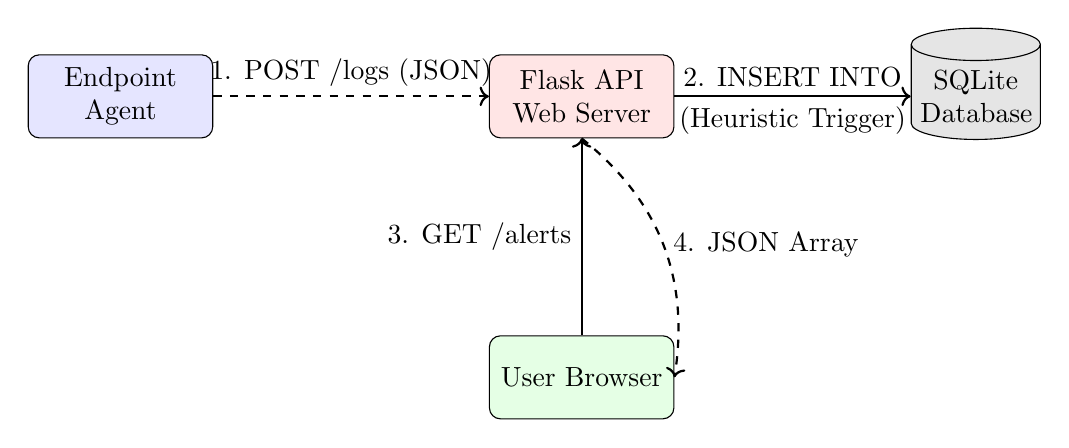
\begin{tikzpicture}[node distance=2.5cm, auto,
            agent/.style={rectangle, draw, fill=blue!10, text width=6em, text centered, rounded corners, minimum height=3em},
            server/.style={rectangle, draw, fill=red!10, text width=6em, text centered, rounded corners, minimum height=3em},
            db/.style={cylinder, draw, shape border rotate=90, aspect=0.25, fill=gray!20, text width=4em, text centered, minimum height=3em},
            client/.style={rectangle, draw, fill=green!10, text width=6em, text centered, rounded corners, minimum height=3em}]
            
        \node [agent] (node1) {Endpoint Agent};
        \node [server, right=of node1, xshift=1cm] (flask) {Flask API Web Server};
        \node [db, right=of flask, xshift=0.5cm] (sqlite) {SQLite Database};
        \node [client, below=of flask] (browser) {User Browser};
        
        % Agent to Server
        \draw[->, thick, dashed] (node1.east) -- node[above] {1. POST /logs (JSON)} (flask.west);
        
        % Server to DB (Write)
        \draw[->, thick] (flask.east) -- node[above] {2. INSERT INTO} node[below] {(Heuristic Trigger)} (sqlite.west);
        
        % Browser to Server (Poll)
        \draw[->, thick] (browser.north) -- node[left] {3. GET /alerts} (flask.south);
        
        % Server to Browser (Response)
        \draw[->, thick, dashed] (flask.south) to[bend left=30] node[right] {4. JSON Array} (browser.east);

    \end{tikzpicture}
    \caption{Unified Modeling Language (UML) structural sequence detailing the full API request lifecycle.}
    \label{fig:uml_seq}
\end{figure}

\section{Database Schema Design Block}
To persistently track the operational history of the network without overwhelming processing overhead or incurring significant licensing costs, a standalone SQLite database engine was permanently integrated directly into the `app.py` wrapper directory structure. 

Crucially, to prevent data concurrency deadlocks during simultaneous logging and querying by multiple users—a notorious weakness in basic SQLite setups deployed across network file systems (NFS)—the Write-Ahead Logging (WAL) pragmas were manually enabled within the `db.py` driver abstraction layer. 

The core schema comprises four critical relational tables linked via explicit foreign keys, establishing strict referential integrity.

\subsection{Relational Entity Mappings}
Table 3-1 presents the schema definition for the primary `alerts` archive, highlighting data types and functional descriptions.

\begin{table}[h]
\centering
\small
\begin{tabularx}{\textwidth}{|l|c|X|}
\hline
\textbf{Field Name} & \textbf{Data Type} & \textbf{Functional Description} \\ \hline
id & INTEGER & Primary Key (Auto-increment format) for the alert incident. \\ \hline
host\_id & INTEGER & Relational Foreign Key structurally linking to the source host in the `hosts` table. \\ \hline
rule\_name & TEXT & The nominal descriptor of the triggered detection heuristic (e.g., ``High CPU Utilization''). \\ \hline
severity & TEXT & Categorical severity ranking constraint: `Low`, `Medium`, `High`. \\ \hline
category & TEXT & Attack vector classification (e.g., `metrics`, `auth`, `process\_list`). \\ \hline
raw\_payload & JSON TEXT & The direct, immutable evidentiary telemetry string extracted verbatim from the original system logs. \\ \hline
status & TEXT & Workflow lifecycle state string identifier: `new`, `handled`, `resolved`. \\ \hline
timestamp & DATETIME & Temporal integer auto-generated on insertion (CURRENT\_TIMESTAMP). \\ \hline
\end{tabularx}
\caption{Detailed database schema mapping for the primary SIEM `alerts` management table.}
\end{table}

\section{Detection Engine Heuristic Logic}
The central intelligence and cognitive processing weight of the SOC ultimately resides in the `detection.py` micro-service. The analytical layer shuns resource-intensive Machine Learning operations in favor of a deterministic, rigid threshold-based calculation script. 

The engine actively unmarshals the incoming JSON transmission and extracts numeric integers corresponding to pre-mapped key-value dictionary combinations.
For example, standard resource anomaly checks iterate through the incoming system payload matrix in real-time. 

\subsection{Pseudo-Code Algorithmic Implementation}
The foundational logic for capturing CPU resource starvation natively is defined algorithmically as follows:

\begin{verbatim}
FUNCTION EvaluateLocalPayload(log_entry, database_rules)
    alerts_queue = []
    
    FOR rule IN database_rules:
        condition_logic = rule.get('logic_syntax')
        operator = condition_logic.get('operator') // e.g., '>', '<', 'contains'
        threshold = condition_logic.get('value')
        
        extracted_metric = ExtractTargetData(log_entry, rule.field)
        
        IF operator == '>' AND Type(extracted_metric) == Integer:
            IF extracted_metric > threshold:
                alerts_queue.Append({
                    'Triggered_Rule': rule.name,
                    'Evidence_Data': log_entry,
                    'Host': log_entry.origin
                })
        
        IF operator == 'contains' AND Type(extracted_metric) == Array:
             IF threshold IN extracted_metric: // Example: 'nmap' IN processes
                  alerts_queue.Append(...)
                  
    RETURN alerts_queue
\end{verbatim}

By architecturally decoupling the Rule Definitions (stored statically as SQL rows) from the Logic Engine execution loop, system administrators receive the distinct strategic advantage of freely updating security parameters globally without necessitating physical modifications or operational downtime to the underlying Python execution environment. This strict topological isolation dramatically increases the long-term maintainability, patchability, and functional modularity of the HomeSOC system.

\begin{figure}[h]
    \centering
    % Placeholder for Sandbox View Screenshot
    \fbox{
        \begin{minipage}{0.8\textwidth}
            \vspace{2cm}
            \begin{center}
                \textit{[PLACEHOLDER: Insert Screenshot of SQL Sandbox Tab UI Dashboard]} \\
                \vspace{0.5cm}
                File: \texttt{sandbox\_execution.png}
            \end{center}
            \vspace{2cm}
        \end{minipage}
    }
    \caption{The SQL analytical sandbox allowing real-time administrative access into the raw relational schema.}
    \label{fig:sandbox_ui}
\end{figure}

\section{REST API Mapping Configuration}
A comprehensive API matrix defines the endpoints interacting with the client-side logic. To formalize backend-frontend separation, Table 3-2 details the defined operational HTTP routing paths.

\begin{table}[h]
\centering
\small
\begin{tabularx}{\textwidth}{|X|c|X|c|}
\hline
\textbf{Endpoint URI Route} & \textbf{Method} & \textbf{Functionality Protocol Description} & \textbf{Auth Needs} \\ \hline
\texttt{/api/heartbeat} & POST & Registers host nodes dynamically into the `hosts` schema table. & None (MVP) \\ \hline
\texttt{/api/logs} & POST & Core telemetry ingestion endpoint executing detection heuristics. & None (MVP) \\ \hline
\texttt{/api/alerts/active} & GET & Real-time fetch sequence feeding the DOM dashboard arrays. & Yes \\ \hline
\texttt{/api/alerts/history} & GET & Retrieves resolved, handled, or suppressed historical alerts. & Yes \\ \hline
\texttt{/api/query} & POST & Direct raw SQLite execution sandbox query endpoint. & Strict Admin \\ \hline
\end{tabularx}
\caption{The structured REST API web routing matrix configuring host and interface communication layers.}
\label{tab:api_maps}
\end{table}

\section{Expanded Theoretical Framework: Database Architecture and SQLite B-Trees}
SQLite ( "S-Q-L-ite",  "sequel-ite") is a free and open-source relational database engine written in the C programming language. It is not a standalone application; rather, it is a library that software developers embed in their applications. As such, it belongs to the family of embedded databases. According to its developers, SQLite is the most widely deployed database engine, as it is used by several of the top web browsers, operating systems, mobile phones, and other embedded systems.
Many programming languages have bindings to the SQLite library. It generally follows PostgreSQL syntax, but does not enforce type checking by default. This means that one can, for example, insert a string into a column defined as an integer. Although it is a lightweight embedded database, SQLite implements most of the SQL standard and the relational model, including transactions and ACID guarantees. However, it omits many features implemented by other databases, such as materialized views and complete support for triggers and ALTER TABLE statements.


== History ==
D. Richard Hipp designed SQLite in the spring of 2000 while working for General Dynamics on contract with the United States Navy. Hipp was designing software used for a damage-control system aboard guided-missile destroyers; the damage-control system originally used HP-UX with an Informix database back-end. SQLite began as a Tcl extension.
In August 2000, version 1.0 of SQLite was released, with storage based on gdbm (GNU Database Manager). In September 2001, SQLite 2.0 replaced gdbm with a custom B-tree implementation, adding transaction capability. In June 2004, SQLite 3.0 added internationalization, manifest typing, and other major improvements, partially funded by America Online. In 2011, Hipp announced his plans to add a NoSQL interface to SQLite, as well as announcing UnQL, a functional superset of SQL designed for document-oriented databases.
SQLite is one of four formats recommended for long-term storage of datasets approved for use by the Library of Congress.


== Design ==
SQLite was designed to allow the program to be operated without installing a database management system or requiring a database administrator. Unlike client–server database management systems, the SQLite engine has no standalone processes with which the application program communicates. Instead, a linker integrates the SQLite library—statically or dynamically—into an application program which uses SQLite's functionality through simple function calls, reducing latency in database operations; for simple queries with little concurrency, SQLite performance profits from avoiding the overhead of inter-process communication.
Due to the serverless design, SQLite applications require less configuration than client–server databases. SQLite is called zero-configuration because configuration tasks such as service management, startup scripts, and password- or GRANT-based access control are unnecessary. Access control is handled through the file-system permissions of the database file. Databases in client–server systems use file-system permissions that give access to the database files only to the daemon process, which handles its locks internally, allowing concurrent writes from several processes.
SQLite stores the entire database, consisting of definitions, tables, indices, and data, as a single cross-platform file, allowing several processes or threads to access the same database concurrently. It implements this simple design by locking the database file during writing. Write access may fail with an error code, or it can be retried until a configurable timeout expires. SQLite read operations can be multitasked, though due to the serverless design, writes can only be performed sequentially. This concurrent access restriction does not apply to temporary tables, and it is relaxed in version 3.7 as write-ahead logging (WAL) enables concurrent reads and writes. Since SQLite has to rely on file-system locks, it is not the preferred choice for write-intensive deployments.
SQLite uses PostgreSQL as a reference platform. "What would PostgreSQL do" is used to make sense of the SQL standard. One major deviation is that, with the exception of primary keys, SQLite does not enforce type checking; the type of a value is dynamic and not strictly constrained by the schema (although the schema will trigger a conversion when storing, if such a conversion is potentially reversible). SQLite strives to follow Postel's rule.


== Features ==
SQLite implements most of the SQL-92 standard for SQL, but lacks some features. For example, it only partially provides triggers and cannot write to views (however, it provides INSTEAD OF triggers that provide this functionality). Its support of ALTER TABLE statements is limited.
SQLite uses an unusual type system for an SQL-compatible DBMS: instead of assigning a type to a column as in most SQL database systems, types are assigned to individual values; in language terms it is dynamically typed. Moreover, it is weakly typed in some of the same ways that Perl is: one can insert a string into an integer column (although SQLite will try to convert the string to an integer first, if the column's preferred type is integer). This adds flexibility to columns, especially when bound to a dynamically typed scripting language. However, the technique is not portable to other SQL products. A common criticism is that SQLite's type system lacks the data integrity mechanism provided by statically typed columns, although it can be emulated with constraints like CHECK(typeof(x)='integer'). In 2021, support for static typing was added through STRICT tables, which enforce datatype constraints for columns.
Tables normally include a hidden rowid index column, which provides faster access. If a table includes an INTEGER PRIMARY KEY column, SQLite will typically optimize it by treating it as an alias for the rowid, causing the contents to be stored as a strictly typed 64-bit signed integer and changing its behavior to be somewhat like an auto-incrementing column. SQLite includes an option to create a table without a rowid column, which can save disk space and improve lookup speed. WITHOUT ROWID tables are required to have a primary key.
SQLite supports foreign key constraints, although they are disabled by default and must be manually enabled with a PRAGMA statement.
Stored procedures are not supported; this is an explicit choice by the developers to favor simplicity, as the typical use case of SQLite is to be embedded inside a host application that can define its own procedures around the database.
SQLite does not have full Unicode support by default for backwards compatibility and due to the size of the Unicode tables, which are larger than the SQLite library. Full support for Unicode case-conversions can be enabled through an optional extension.
SQLite supports full-text search through its FTS5 loadable extension, which allows users to efficiently search for a keyword in a large number of documents similar to how search engines search webpages.
SQLite includes support for working with JSON through its json1 extension, which is enabled by default since 2021. SQLite's JSON functions can handle JSON5 syntax since 2023. In 2024, SQLite added support for JSONB, a binary serialization of SQLite's internal representation of JSON. Using JSONB allows applications to avoid having to parse the JSON text each time it is processed and saves a small amount of disk space.
In May 2025, the 25th‑anniversary release SQLite 3.50.0 introduced additional features, including new Unicode functions (unistr() and unistr\_quote()), a new API (sqlite3\_setlk\_timeout()) for setting lock timeouts, improved command‑line tools and rsync utility enhancements, and optimized JSONB.
The maximum supported size for an SQLite database file is 281 terabytes.


== Development and distribution ==
SQLite's code is hosted with Fossil, a distributed version control system that uses SQLite as a local cache for its non-relational database format, and SQLite's SQL as an implementation language.
SQLite is public domain, but not "open-contribution", with the website stating "the project does not accept patches from people who have not submitted an affidavit dedicating their contribution into the public domain." Instead of a code of conduct, the founders have adopted a code of ethics based on the Rule of St. Benedict.
A standalone command-line shell program called sqlite3 is provided in SQLite's distribution. It can be used to create a database, define tables, insert and change rows, run queries and manage an SQLite database file. It also serves as an example for writing applications that use the SQLite library.
SQLite uses automated regression testing prior to each release. Over 2 million tests are run as part of a release's verification. The SQLite library has 156,000 lines of source code, while all the test suites combined add up to 92 million lines of test code. SQLite's tests simulate a number of exceptional scenarios, such as power loss and I/O errors, in addition to testing the library's functionality. Starting with the August 10, 2009 release of SQLite 3.6.17, SQLite releases have 100\% branch test coverage, one of the components of code coverage. SQLite has four different test harnesses: the original public-domain TCL tests, the proprietary C-language TH3 test suite, the SQL Logic Tests, which check SQLite against other SQL databases, and the dbsqlfuzz proprietary fuzzing engine.


== Notable uses ==


=== Operating systems ===
SQLite is included by default in:

Android
BlackBerry 10 OS
Fedora Linux where it is used by the rpm core package management system
FreeBSD where starting with 10-RELEASE version in January 2014, it is used by the core package management system.
illumos
iOS
Mac OS X 10.4 onwards (Apple adopted it as an option in macOS's Core Data API from the original implementation)
Maemo
MeeGo
MorphOS 3.10 onwards
NetBSD
NixOS where it is used by the Nix core package management system
Red Hat Enterprise Linux where it is used in the same way as Fedora, from which Red Hat Enterprise Linux is derived
Solaris 10 where the Service Management Facility database is serialized for booting.
Symbian OS
Tizen
webOS
Windows 10 onwards


=== Middleware ===
ADO.NET adapter, initially developed by Robert Simpson, is maintained jointly with the SQLite developers since April 2010.
ODBC driver has been developed and is maintained separately by Christian Werner. Werner's ODBC driver is the recommended connection method for accessing SQLite from OpenOffice.org.
COM (ActiveX) wrapper making SQLite accessible on Windows to scripted languages such as JScript and VBScript. This adds SQLite database capabilities to HTML Applications (HTA).


=== Web browsers ===
The browsers Google Chrome, Opera, Safari and the Android Browser all allow for storing information in, and retrieving it from, an SQLite database within the browser, using the official SQLite Wasm (WebAssembly) build, or using the Web SQL Database technology, although the latter is becoming deprecated (namely superseded by SQLite Wasm or by IndexedDB). Internally, these Chromium based browsers use SQLite databases for storing configuration data like site visit history, cookies, download history etc.
Mozilla Firefox and Mozilla Thunderbird store a variety of configuration data (bookmarks, cookies, contacts etc.) in internally managed SQLite databases. Until Firefox version 57 ("Firefox Quantum"), there was a third-party add-on that used the API supporting this functionality to provide a user interface for managing arbitrary SQLite databases.
Several third-party add-ons can make use of JavaScript APIs to manage SQLite databases.


=== Web application frameworks ===
Symfony
Laravel
Bugzilla
Django's default database management system
Drupal
Trac
Ruby on Rails's default database management system
web2py


=== Others ===
Adobe Systems uses SQLite as its file format in Adobe Lightroom, a standard database in Adobe AIR, and internally within Adobe Reader.
Apple Photos uses SQLite internally.
Audacity uses SQLite as its file format, as of version 3.0.0.
Evernote uses SQLite to store its local database repository in Windows.
Skype
WhatsApp
The Service Management Facility, used for service management within the Solaris and OpenSolaris operating systems
Dropbox client software
Intuit uses SQLite in QuickBooks and TurboTax
McAfee Antivirus
Flame (malware)
BMW iDrive satellite navigation system
TomTom GPS systems, for the NDS map data
Proxmox VE - Proxmox Cluster File System (pmxcfs)
Bentley Systems MicroStation
Bosch car multimedia systems
Airbus A350 flight system
Quicken Essentials and later versions of Quicken for Mac
Python standard library
Xojo IDE


== See also ==

Ordered key–value store
Comparison of relational database management systems
List of relational database management systems
MySQL
SpatiaLite


== Notes ==

A relational database (RDB) is a database  based on the relational model of data, as proposed by E. F. Codd in 1970.
A Relational Database Management System (RDBMS) is a type of database management system that stores data in a structured format using rows and columns.
Many relational database systems are equipped with the option of using SQL (Structured Query Language) for querying and updating the database.


== History ==
The concept of relational database was defined by E. F. Codd at IBM in 1970. Codd introduced the term relational in his research paper "A Relational Model of Data for Large Shared Data Banks". In this paper and later papers, he defined what he meant by relation. One well-known definition of what constitutes a relational database system is composed of Codd's 12 rules.
However, no commercial implementations of the relational model conform to all of Codd's rules, so the term has gradually come to describe a broader class of database systems, which at a minimum:

Present the data to the user as relations (a presentation in tabular form, i.e. as a collection of tables with each table consisting of a set of rows and columns);
Provide relational operators to manipulate the data in tabular form.
In 1974, IBM began developing System R, a research project to develop a prototype RDBMS.
The first system sold as an RDBMS was Multics Relational Data Store (June 1976). Oracle was released in 1979 by Relational Software, now Oracle Corporation. Ingres and IBM BS12 followed. Other examples of an RDBMS include IBM Db2, SAP Sybase ASE, and Informix. In 1984, the first RDBMS for Macintosh began being developed, code-named Silver Surfer, and was released in 1987 as 4th Dimension and known today as 4D.
The first systems that were relatively faithful implementations of the relational model were from:

University of Michigan – Micro DBMS (1969)
Massachusetts Institute of Technology (1971)
IBM UK Scientific Centre at Peterlee – IS1 (1970–72), and its successor, PRTV (1973–79).
The most common definition of an RDBMS is a product that presents a view of data as a collection of rows and columns, even if it is not based strictly upon relational theory. By this definition, RDBMS products typically implement some but not all of Codd's 12 rules.
A second school of thought argues that if a database does not implement all of Codd's rules (or the current understanding on the relational model, as expressed by Christopher J. Date, Hugh Darwen and others), it is not relational. This view, shared by many theorists and other strict adherents to Codd's principles, would disqualify most DBMSs as not relational. For clarification, they often refer to some RDBMSs as truly-relational database management systems (TRDBMS), naming others pseudo-relational database management systems (PRDBMS). 
As of 2009, most commercial relational DBMSs employ SQL as their query language.
Alternative query languages have been proposed and implemented, notably the pre-1996 implementation of Ingres QUEL.


== Relational model ==

A relational model organizes data into one or more tables (or "relations") of columns and rows, with a unique key identifying each row. Rows are also called records or tuples. Columns are also called attributes. Generally, each table/relation represents one "entity type" (such as customer or product). The rows represent instances of that type of entity (such as "Lee" or "chair") and the columns represent values attributed to that instance (such as address or price).
For example, each row of a class table corresponds to a class, and a class corresponds to multiple students, so the relationship between the class table and the student table is "one to many"


== Keys ==
Each row in a table has its own unique key. Rows in a table can be linked to rows in other tables by adding a column for the unique key of the linked row (such columns are known as foreign keys). Codd showed that data relationships of arbitrary complexity can be represented by a simple set of concepts.
Part of this processing involves consistently being able to select or modify one and only one row in a table. Therefore, most physical implementations have a unique primary key (PK) for each row in a table. When a new row is written to the table, a new unique value for the primary key is generated; this is the key that the system uses primarily for accessing the table. System performance is optimized for PKs. Other, more natural keys may also be identified and defined as alternate keys (AK). Often several columns are needed to form an AK (this is one reason why a single integer column is usually made the PK). Both PKs and AKs have the ability to uniquely identify a row within a table. Additional technology may be applied to ensure a unique ID across the world, a globally unique identifier, when there are broader system requirements.
The primary keys within a database are used to define the relationships among the tables. When a PK migrates to another table, it becomes a foreign key (FK) in the other table. When each cell can contain only one value and the PK migrates into a regular entity table, this design pattern can represent either a one-to-one or one-to-many relationship. Most relational database designs resolve many-to-many relationships by creating an additional table that contains the PKs from both of the other entity tables –  the relationship becomes an entity; the resolution table is then named appropriately and the two FKs are combined to form a PK. The migration of PKs to other tables is the second major reason why system-assigned integers are used normally as PKs; there is usually neither efficiency nor clarity in migrating a bunch of other types of columns.


=== Relationships ===
Relationships are a logical connection between different tables (entities), established on the basis of interaction among these tables. These relationships can be modelled as an entity-relationship model.


== Transactions ==
In order for a database management system (DBMS) to operate efficiently and accurately, it must use ACID transactions.


== Stored procedures ==
Part of the programming within an RDBMS is accomplished using stored procedures (SPs). Often procedures can be used to greatly reduce the amount of information transferred within and outside of a system. For increased security, the system design may grant access to only the stored procedures and not directly to the tables. Fundamental stored procedures contain the logic needed to insert new and update existing data. More complex procedures may be written to implement additional rules and logic related to processing or selecting the data.


== Terminology ==

The relational database was first defined in June 1970 by Edgar Codd, of IBM's San Jose Research Laboratory. Codd's view of what qualifies as an RDBMS is summarized in Codd's 12 rules. A relational database has become the predominant type of database. Other models besides the relational model include the hierarchical database model and the network model.
The table below summarizes some of the most important relational database terms and the corresponding SQL term:


== Relations or tables ==

In a relational database, a relation is a set of tuples that have the same attributes. A tuple usually represents an object and information about that object. Objects are typically physical objects or concepts. A relation is usually described as a table, which is organized into rows and columns. All the data referenced by an attribute are in the same domain and conform to the same constraints.
The relational model specifies that the tuples of a relation have no specific order and that the tuples, in turn, impose no order on the attributes. Applications access data by specifying queries, which use operations such as select to identify tuples, project to identify attributes, and join to combine relations. Relations can be modified using the insert, delete, and update operators. New tuples can supply explicit values or be derived from a query. Similarly, queries identify tuples for updating or deleting.
Tuples by definition are unique. If the tuple contains a candidate or primary key then obviously it is unique; however, a primary key need not be defined for a row or record to be a tuple. The definition of a tuple requires that it be unique, but does not require a primary key to be defined. Because a tuple is unique, its attributes by definition constitute a superkey.


== Base and derived relations ==

\chapter{Methodology and Requirements}

\section{Methodology and Toolchain Selection}
In physically constructing the HomeSOC application, a rapid, iterative agile development methodology was actively integrated. The overarching project timeline was aggressively sequenced into distinct, segmented, programmable objectives, meticulously prioritizing the core local data processing loop prior to engineering the eventual full-scale cloud deployment mechanism. This structural phase formally specifies the critical path toolchain selected for conceptualizing and finalizing the analytical system architecture.

\subsection{Back-End Programming Languages}
The foundational logic processing, ingestion API scripting, and physical agent polling sequences were entirely formulated utilising Python 3 (specifically interpreted under Python 3.8+ versions). This deliberate selection was primarily necessitated by Python's unparalleled ecosystem of mature, cross-platform external libraries combined with its native syntactical brevity, which enables rapid prototyping of computational architectures. 

Unlike heavy, compiled binaries derived from C or Go, which require specific architectural build environments, Python's ubiquitous interpreter nature ensures maximum logistical distribution across heterogeneous network spaces (running invariably on legacy Windows machines, UNIX-based Linux distributions, and containerised micro-services). The built-in `json` string encoder mapped telemetry flawlessly without requiring third-party serializers. Furthermore, the reliance on the third-party `psutil` (Process and System Utilities) library facilitated seamless, hardware-agnostic metric scraping of deep systemic constants (e.g., CPU frequency thresholds, active PID enumeration) isolated entirely from native operating systems shells.

\begin{figure}[h]
    \centering
    % Placeholder for Agent Output Screenshot
    \fbox{
        \begin{minipage}{0.6\textwidth}
            \vspace{2cm}
            \begin{center}
                \textit{[PLACEHOLDER: Insert Terminal Output Screenshot of the Python Host Agent actively scraping telemetry metrics (e.g. `python agent.py` command line output)]} \\
                \vspace{0.5cm}
                File: \texttt{agent\_console\_log.png}
            \end{center}
            \vspace{2cm}
        \end{minipage}
    }
    \caption{Expected native console output from the deployed telemetry agent operating successfully on a host node.}
    \label{fig:agent_console}
\end{figure}

\subsection{Microservices Framework Integration}
To accurately synthesize and bridge the localized agent traffic to the centralised backend, the Flask micro-framework routing logic was heavily utilized. This selection was diametrically opposed to heavier web administration paradigms like the Django MVC system, which explicitly imposes rigid monolithic configurations onto the project structure. 

Flask provided the absolute minimalistic flexibility essential for writing ultra-fast, highly targeted REST APIs capable of concurrently ingesting tens of thousands of localized TCP/IP telemetry strings devoid of excess computational bloat. 

\subsection{Data Persistence and Storage Mediums}
Data storage persistence natively relied on a robust, localized, serverless SQLite (Structured Query Language) installation. The conscious implementation decision to systematically abstain from deploying a sprawling relational database management system (RDBMS) like MySQL or a Document-Store NoSQL engine like MongoDB was principally dictated by the project's inviolable core tenet: extreme accessibility. The HomeSOC architecture had to absolutely remain logistically undemanding and universally executable across low-powered or legacy hardware environments quintessential to home lab networks.

However, as the project scaled from local testing to concurrent testing, the database inevitably confronted severe performance barriers and "I/O lock" anomalies when positioned within a simulated cloud filesystem (specifically, encountering heavy Network File System (NFS) input overhead queues). The root architecture was subsequently refined by adopting SQLite's Write-Ahead Logging (Pragmatic parameter `journal\_mode=WAL`) overriding the default legacy rollback journaling system to optimize multithreaded ingress.

\subsection{Front-End Aesthetics and UI Frameworks}
The aesthetic ambition behind the dashboard was the synthesis of a premium, corporate-grade graphical user interface (GUI) coupled with non-blocking, zero-latency visual polling. Consequently, standard, non-compiled web technologies dominated the UI specification. 

Vanilla ECMAScript JavaScript provided instantaneous Document Object Model (DOM) manipulations directly via the browser's asynchronous `fetch` integration method API. The UI eschews framework build steps (React, Node, Webpack). For styling rendering, complex CSS3 grid mechanics, specifically adopting the modern OKLCH hue parameter colour space calculation system, delivered robust dark-mode aesthetics that facilitate the projection of dynamic scalable interface elements natively.

Ultimately, achieving functional redundancy, the total source code repository underwent a critical final migration from local `localhost` network adapters (127.0.0.1 loopbacks) out into a full-scale production-grade cloud container infrastructure, orchestrated exclusively through the PythonAnywhere web-hosting utility provider.

\section{Software and Hardware Requirement Analysis}
Prior to programmatic execution, exhaustive conceptual and physical analyses establishing specific hardware dependencies and software interpreter prerequisites were systematically finalized to guarantee overarching viability metrics when scaling across diverse client networks.

\subsection{Endpoint Hardware Specifications}
A distinguishing novelty of the proposed local SOC application compared to competing enterprise products is its sheer nominal resource footprint. The requirements actively define computational scarcity:

\begin{enumerate}
    \item \textbf{Monitored Agent Endpoints:} The nodes can encompass any physical or hypervisor-virtual machine actively running a modern kernel operating system (distros ranging from Debian/Ubuntu Linux, Microsoft Windows 10/11, or macOS Big Sur upwards). The node mandates a restrictive minimum of merely 256MB allocated RAM and an operational standard Network Interface Card (NIC). No dedicated compute logic clusters (GPUs) are required, firmly placing the agent parameters within the capabilities of hardware as inexpensive and minimal as an ARM-based Raspberry Pi.
    \item \textbf{Analytical Central Server (Hybrid/Static):} When hosting the backend statically on physical hardware, the machine merely requires the presence of a baseline Consumer Dual-Core Processor (x86 or ARM64 instruction set), 1GB of continuous functional system memory, and a bare minimum of 5GB of localized storage capacity strictly dedicated to preserving historical tabular database logging records (`soc\_db.sqlite`). A static IP lease and continuous stable routing are explicitly crucial.
\end{enumerate}

\subsection{Software Stack Requirements}
Given the heavy dependence on OS-agnostic frameworks, the programmatic requisites are deliberately universalized:
\begin{enumerate}
    \item \textbf{Scripting Interpreter:} Python version 3.8, natively required in order to support executing precise f-string format literals, syntax iteration functions in tuples, and concurrent library modules deployed across the ingestion routing sequences.
    \item \textbf{Network Dependency Tree:} A virtualized shell environment `venv` physically retaining the package library list documented inside `requirements.txt`. Essential installation prerequisites included `Flask`, `Flask-Cors` (resolving complex cross-origin resource sharing blockages), `psutil`, `requests`, and potentially `mysql-connector-python` as a redundancy mechanism.
    \item \textbf{Analyst Client Display Access:} A highly standardized WebKit or Chromium-based modern visual browser.
    \item \textbf{Application Deployment Environment:} A functional PythonAnywhere WSGI configuration web application instance preconfigured over Ubuntu 22.04 LTS equipped natively with accessible secure bash consoles.
\end{enumerate}

\section{Methodology Table Synthesization}
The final toolchain assembly mapping represented systematically in Table 4-1 accurately reflects the strategic prioritization of security insight visibility combined with drastic systemic simplification over abstract operational complexity.

\begin{table}[h]
\centering
\small
\begin{tabularx}{\textwidth}{|X|X|X|}
\hline
\textbf{Architectural Category} & \textbf{Tool / Library Utilized} & \textbf{Strategic Selection Justification Matrix} \\ \hline
Backend API Framework & Python / Flask & Zero bloat, maximal REST integration flexibility, JSON ease. \\ \hline
System Telemetry Extractor & psutil Module & Hardware-agnostic deep systemic kernel scraping logic. \\ \hline
Data Persistence Archival & SQLite3 (WAL pragmas) & Total zero-configuration, standalone executable serverless storage format. \\ \hline
Production Cloud Infrastructure & PythonAnywhere & Persistent, universally accessible TLS terminal presence. \\ \hline
Frontend Interface Logic & Pure Vanilla JS / CSS3 & Infinite backward DOM compatibility array producing sub-millisecond reaction speeds. \\ \hline
\end{tabularx}
\caption{Comprehensive breakdown of the fundamental technology stack parameters dictating the HomeSOC framework construction.}
\label{tab:method_stack}
\end{table}

\section{Verification Specifications - Bruteforce Mathematical Analytical Plan}
Analytical project milestones heavily dictated that the completed ingestion API must faultlessly accept variable JSON payloads without dropping packets due to HTTP payload congestion overload. The system essentially must guarantee returning a standard `HTTP 200 OK` succession code or a strict `HTTP 400 Bad Request` verification error immediately if fundamental structural parsing mechanisms internally failed. 

To formally verify design adherence against these rigorous specifications, the testing phase integrated a dedicated, heavily multithreaded Python stress-testing script module specifically coded as `stress\_test.py`. This script was purposefully and aggressively utilized to brute-force the localized central API endpoint by computationally simulating an artificial multitude of heterogeneous nodes launching overlapping, consecutive mock attacks. Simulated parameters included generating massive synthesized CPU frequency throttling warnings, creating dummy SSH authentication login sequence denials, and embedding fake network footprint scanning payloads containing literal string variables commonly mapping to hostile binaries (`xmrig` cryptocurrency executable patterns and `nmap` reconnaissance routines). 

The defined verification criteria demanded compliance metrics indicating that:
\begin{itemize}
    \item The relational schema correctly mapped and appended 100\% of the simulated telemetry traffic logs seamlessly devoid of connection reset flags.
    \item The fundamental `detection.py` logical arithmetic engine correctly parsed JSON dictionaries and flawlessly aligned simulated mathematical telemetry values successfully against static pre-established numerical algorithmic thresholds encoded into the rules table.
    \item The primary analyst reporting dashboard effectively polled the resultant changes sequentially over network parameters and visibly assigned physical styling classifications of `Low`, `Medium`, and `High` severity tags to the specific anomalies accurately without missing data arrays. 
    \item The GUI interactive notification alert system logically and systematically strictly observed distinct threshold gating logic patterns (e.g. perpetually silencing modal pop-up alarms for minimal `Low` warnings, effectively constraining visual noise, whilst immediately and aggressively asserting graphical dominance and stacking arrays to demand interactive human operator acknowledgment strictly for prioritized `High` warnings).
\end{itemize}
This precise verification specification structure functionally informed the subsequent complex programmatic implementation mapping documented precisely in Chapter 5.

\section{Expanded Theoretical Framework: Software Development Lifecycles}
A software development process prescribes a process for developing software. It typically divides an overall effort into smaller steps or sub-processes that are intended to ensure high-quality results. The process may describe specific deliverables – artifacts to be created and completed. 
Although not strictly limited to it, software development process often refers to the high-level process that governs the development of a software system from its beginning to its end of life – known as a methodology, model or framework. The system development life cycle (SDLC) describes the typical phases that a development effort goes through from the beginning to the end of life for a system – including a software system. A methodology prescribes how engineers go about their work in order to move the system through its life cycle. A methodology is a classification of processes or a blueprint for a process that is devised for the SDLC. For example, many processes can be classified as a spiral model.
Software process and software quality are closely interrelated; some unexpected facets and effects have been observed in practice.


== Methodology ==
The SDLC drives the definition of a methodology in that a methodology must address the phases of the SDLC. Generally, a methodology is designed to result in a high-quality system that meets or exceeds expectations (requirements) and is delivered on time and within budget even though computer systems can be complex and integrate disparate components. Various methodologies have been devised, including waterfall, spiral, agile, rapid prototyping, incremental, and synchronize and stabilize.
A major difference between methodologies is the degree to which the phases are sequential vs. iterative. Agile methodologies, such as XP and scrum, focus on lightweight processes that allow for rapid changes. Iterative methodologies, such as Rational Unified Process and dynamic systems development method, focus on stabilizing project scope and iteratively expanding or improving products. Sequential or big-design-up-front (BDUF) models, such as waterfall, focus on complete and correct planning to guide larger projects and limit risks to successful and predictable results. Anamorphic development is guided by project scope and adaptive iterations. In scrum, for example, one could say a single user story goes through all the phases of the SDLC within a two-week sprint. By contrast the waterfall methodology, where every business requirement is translated into feature/functional descriptions which are then all implemented typically over a period of months or longer.
A project can include both a project life cycle (PLC) and an SDLC, which describe different activities. According to Taylor (2004), "the project life cycle encompasses all the activities of the project, while the systems development life cycle focuses on realizing the product requirements".


=== History ===
The term SDLC is often used as an abbreviated version of SDLC methodology. Further, some use SDLC and traditional SDLC to mean the waterfall methodology.
According to Elliott (2004), SDLC "originated in the 1960s, to develop large scale functional business systems in an age of large scale business conglomerates. Information systems activities revolved around heavy data processing and number crunching routines". The structured systems analysis and design method (SSADM) was produced for the UK government Office of Government Commerce in the 1980s. Ever since, according to Elliott (2004), "the traditional life cycle approaches to systems development have been increasingly replaced with alternative approaches and frameworks, which attempted to overcome some of the inherent deficiencies of the traditional SDLC". The main idea of the SDLC has been "to pursue the development of information systems in a very deliberate, structured and methodical way, requiring each stage of the life cycle––from the inception of the idea to delivery of the final system––to be carried out rigidly and sequentially" within the context of the framework being applied.
Other methodologies were devised later:

1970s
Structured programming since 1969
Cap Gemini SDM, originally from PANDATA, the first English translation was published in 1974. SDM stands for System Development Methodology
1980s
Structured systems analysis and design method (SSADM) from 1980 onwards
Information Requirement Analysis/Soft systems methodology
1990s
Object-oriented programming (OOP) developed in the early 1960s and became a dominant programming approach during the mid-1990s
Rapid application development (RAD), since 1991
Dynamic systems development method (DSDM), since 1994
Scrum, since 1995
Team software process, since 1998
Rational Unified Process (RUP), maintained by IBM since 1998
Extreme programming, since 1999
2000s
Agile Unified Process (AUP) maintained since 2005 by Scott Ambler
Disciplined agile delivery (DAD) Supersedes AUP
2010s
Scaled Agile Framework (SAFe)
Large-Scale Scrum (LeSS)
DevOps
Since DSDM in 1994, all of the methodologies on the above list except RUP have been agile methodologies - yet many organizations, especially governments, still use pre-agile processes (often waterfall or similar). 


=== Examples ===
The following are notable methodologies somewhat ordered by popularity.

Agile
Agile software development refers to a group of frameworks based on iterative development, where requirements and solutions evolve via collaboration between self-organizing cross-functional teams. The term was coined in the year 2001 when the Agile Manifesto was formulated.

Waterfall
The waterfall model is a sequential development approach, in which development flows one-way (like a waterfall) through the SDLC phases.

Spiral
In 1988, Barry Boehm published a software system development spiral model, which combines key aspects of the waterfall model and  rapid prototyping, in an effort to combine advantages of  top-down and bottom-up concepts. It emphases a key area many felt had been neglected by other methodologies: deliberate iterative risk analysis, particularly suited to large-scale complex systems.

Incremental
Various methods combine linear and iterative methodologies, with the primary objective of reducing inherent project risk by breaking a project into smaller segments and providing more ease-of-change during the development process.

Prototyping
Software prototyping is about creating prototypes, i.e. incomplete versions of the software program being developed.

Rapid
Rapid application development (RAD) is a methodology which favors iterative development and the rapid construction of prototypes instead of large amounts of up-front planning. The "planning" of software developed using RAD is interleaved with writing the software itself. The lack of extensive pre-planning generally allows software to be written much faster and makes it easier to change requirements.

Shape Up
Shape Up is a software development approach introduced by Basecamp in 2018. It is a set of principles and techniques that Basecamp developed internally to overcome the problem of projects dragging on with no clear end. Its primary target audience is remote teams. Shape Up has no estimation and velocity tracking, backlogs, or sprints, unlike waterfall, agile, or scrum. Instead, those concepts are replaced with appetite, betting, and cycles. As of 2022, besides Basecamp, notable organizations that have adopted Shape Up include UserVoice and Block.

Chaos
Chaos model has one main rule: always resolve the most important issue first.

Incremental funding
Incremental funding methodology - an iterative approach.

Lightweight
Lightweight methodology - a general term for methods that only have a few rules and practices.

Agile software development is an umbrella term for approaches to developing software that reflect the values and principles agreed upon by The Agile Alliance, a group of 17 software practitioners, in 2001. As documented in their Manifesto for Agile Software Development, the practitioners value: 

Individuals and interactions over processes and tools
Working software over comprehensive documentation
Customer collaboration over contract negotiation
Responding to change over following a plan
The practitioners cite inspiration from new practices at the time including extreme programming, scrum, dynamic systems development method, adaptive software development, and being sympathetic to the need for an alternative to documentation-driven, heavyweight software development processes.
Many software development practices emerged from the agile mindset. These agile-based practices, sometimes called Agile (with a capital A), include requirements, discovery, and solutions improvement through the collaborative effort of self-organizing and cross-functional teams with their customer(s)/end user(s).
While there is much anecdotal evidence that the agile mindset and agile-based practices improve the software development process, the empirical evidence is limited and less than conclusive.


== History ==
Iterative and incremental software development methods can be traced back as early as 1957, with evolutionary project management and adaptive software development emerging in the early 1970s.
During the 1990s, a number of lightweight software development methods evolved in reaction to the prevailing heavyweight methods (often referred to collectively as waterfall) that critics described as overly regulated, planned, and micromanaged. These lightweight methods included rapid application development (RAD), from 1991; the unified process (UP) and dynamic systems development method (DSDM), both from 1994; Scrum, from 1995; Crystal Clear and extreme programming (XP), both from 1996; and feature-driven development (FDD), from 1997. Although these all originated before the publication of the Agile Manifesto, they are now collectively referred to as agile software development methods.
Already since 1991 similar changes had been underway in manufacturing and management thinking derived from lean management.
In 2001, seventeen software developers met at a resort in Snowbird, Utah to discuss lightweight development methods. They were Kent Beck (Extreme Programming), Ward Cunningham (Extreme Programming), Dave Thomas (Pragmatic Programming, Ruby), Jeff Sutherland (Scrum), Ken Schwaber (Scrum), Jim Highsmith (Adaptive Software Development), Alistair Cockburn (Crystal), Robert C. Martin (SOLID), Mike Beedle (Scrum), Arie van Bennekum, Martin Fowler (OOAD and UML), James Grenning, Andrew Hunt (Pragmatic Programming, Ruby), Ron Jeffries (Extreme Programming), Jon Kern, Brian Marick (Ruby, Test-driven development), and Steve Mellor (OOA). The group, The Agile Alliance, published the Manifesto for Agile Software Development.
In 2005, a group headed by Cockburn and Highsmith wrote an addendum of project management principles, the PM Declaration of Interdependence, to guide software project management according to agile software development methods.
In 2009, a group working with Martin wrote an extension of software development principles, the Software Craftsmanship Manifesto, to guide agile software development according to professional conduct and mastery.
In 2011, the Agile Alliance created the Guide to Agile Practices (renamed the Agile Glossary in 2016), an evolving open-source compendium of the working definitions of agile practices, terms, and elements, along with interpretations and experience guidelines from the worldwide community of agile practitioners.


== Values and principles ==


=== Values ===
The manifesto for agile software development reads:
We are uncovering better ways of developing software by doing it and helping others do it. Through this work we have come to value:

  Individuals and interactions over processes and tools 
  Working software over comprehensive documentation 
  Customer collaboration over contract negotiation 
  Responding to change over following a plan 
That is, while there is value in the items on the right, we value the items on the left more.
Scott Ambler explained:

Tools and processes are important, but it is more important to have competent people working together effectively.
Good documentation is useful in helping people to understand how the software is built and how to use it, but the main point of development is to create software, not documentation.
A contract is important but is not a substitute for working closely with customers to discover what they need.
A project plan is important, but it must not be too rigid to accommodate changes in technology or the environment, stakeholders' priorities, and people's understanding of the problem and its solution.
Introducing the manifesto on behalf of the Agile Alliance, Jim Highsmith said,

The Agile movement is not anti-methodology, in fact many of us want to restore credibility to the word methodology. We want to restore a balance. We embrace modeling, but not in order to file some diagram in a dusty corporate repository. We embrace documentation, but not hundreds of pages of never-maintained and rarely-used tomes. We plan, but recognize the limits of planning in a turbulent environment. Those who would brand proponents of XP or SCRUM or any of the other Agile Methodologies as "hackers" are ignorant of both the methodologies and the original definition of the term hacker.


=== Principles ===
The values are based on these principles:

Customer satisfaction by early and continuous delivery of valuable software.
Welcome changing requirements, even in late development.
Deliver working software frequently (weeks rather than months).
Close, daily cooperation between business people and developers.
Projects are built around motivated individuals, who should be trusted.
Face-to-face conversation is the best form of communication (co-location).
Working software is the primary measure of progress.
Sustainable development, able to maintain a constant pace.
Continuous attention to technical excellence and good design.
Simplicity—the art of maximizing the amount of work not done—is essential.
Best architectures, requirements, and designs emerge from self-organizing teams.
Regularly, the team reflects on how to become more effective, and adjusts accordingly.


== Overview ==


=== Iterative, incremental, and evolutionary ===
Most agile development methods break product development work into small increments that minimize the amount of up-front planning and design. Iterations, or sprints, are short time frames (timeboxes) that typically last from one to four weeks. Each iteration involves a cross-functional team working in all functions: planning, analysis, design, coding, unit testing, and acceptance testing. At the end of the iteration a working product is demonstrated to stakeholders. This minimizes overall risk and allows the product to adapt to changes quickly. An iteration might not add enough functionality to warrant a market release, but the goal is to have an available release (with minimal bugs) at the end of each iteration. Through incremental development, products have room to "fail often and early" throughout each iterative phase instead of drastically on a final release date. Multiple iterations might be required to release a product or new features. Working software is the primary measure of progress.


=== Efficient and face-to-face communication ===
The 6th principle of the agile manifesto for software development states, "The most efficient and effective method of conveying information to and within a development team is face-to-face conversation". The manifesto, written in 2001 when video conferencing was not widely used, states this in relation to the communication of information, not necessarily that a team should be co-located.
The principle of co-location is that co-workers on the same team should be situated together to better establish the identity as a team and to improve communication. This enables face-to-face interaction, ideally in front of a whiteboard, that reduces the cycle time typically taken when questions and answers are mediated through phone, persistent chat, wiki, or email. With the widespread adoption of remote working during the COVID-19 pandemic and changes to tooling, more studies have been conducted around co-location and distributed working which show that co-location is increasingly less relevant.
No matter which development method is followed, every team should include a customer representative (known as product owner in Scrum). This representative is agreed by stakeholders to act on their behalf and makes a personal commitment to being available for developers to answer questions throughout the iteration. At the end of each iteration, the project stakeholders together with the customer representative review progress and re-evaluate priorities with a view to optimizing the return on investment (ROI) and ensuring alignment with customer needs and company goals. The importance of stakeholder satisfaction, detailed by frequent interaction and review at the end of each phase, is why the approach is often denoted as a customer-centered methodology.


==== Information radiator ====
In agile software development, an information radiator is a (normally large) physical display, board with sticky notes or similar, located prominently near the development team, where passers-by can see it. It presents an up-to-date summary of the product development status. A build light indicator may also be used to inform a team about the current status of their product development.


=== Very short feedback loop and adaptation cycle ===
A common characteristic in agile software development is the daily stand-up (known as daily scrum in the Scrum framework). In a brief session (e.g., 15 minutes), team members review collectively how they are progressing toward their goal and agree whether they need to adapt their approach. To keep to the agreed time limit, teams often use simple coded questions (such as what they completed the previous day, what they aim to complete that day, and whether there are any impediments or risks to progress), and delay detailed discussions and problem resolution until after the stand-up.

\chapter{Implementation and Testing}

\section{Implementation Details Overview}
The software engineering and functional codebase development of the HomeSOC application necessitated explicit computational translation of the structured agile methodologies previously outlined into entirely executable Python arrays and browser-compliant script objects. This comprehensive section sequentially deconstructs the precise programmatic execution flow detailing precisely how the individual functional boundary layers—the Edge Host Agent scripts, the Heuristic Detection computational engine, the complex Graphical Web Dashboard interface controllers—were systematically produced, including precise analysis pertaining to the eventual transition out of theoretical local bounds into production cloud implementation topologies.

\subsection{Endpoint Host Agent Telemetry Scraping Loop}
The functional Host Agent element was natively coded predominantly as an independent, perpetually daemonised Python 3 interpreter process executable on target client node hardware platforms. The initial operational protocol executed mathematically by the agent script instantiates a formal network registration. Activating a persistent system heartbeat mechanism, it immediately registers the hardware node against the active Flask application's backend `/api/heartbeat` listener endpoint via an authenticated, authenticated REST call. 

This specific outgoing programmatic `POST` request effectively packages and transmits a structured nested Python dictionary automatically serialized into a uniform JSON character string. This string dynamically declares essential physical environmental variables: the unique local hardware node execution `hostname`, the active routing IPv4 routing address metadata (`ip\_address`), combined with granular, version-tagged kernel string classifications extracting the specific OS metadata (`os`).  

Following immediate unencrypted transmission and subsequent SQL successful registration confirmation logic passed from the server loopback, the agent script activates a persistent recurring statistical data-loop mechanism running concurrently on a sleep-interval delay. Invoking the universally deployed hardware-agnostic Python module `psutil`, the logic block continually aggregates operational vectors including realtime systemic CPU computation usage fractional percentages, instantaneous virtual memory RAM utilisation capacity over-commitment, and cumulative block input/output operational latency fractions running into the system cache logic block. 

Concurrently running isolated threads map standard log character configurations directly against localized, native physical kernel security log plaintext flat-files (notably Linux distributions operating `auth.log` or SystemD Journald interfaces), specifically scanning via rudimentary list indexing combinations for specific string literals categorically characteristic of violent, persistent unauthorized system access authentication traversal failures (e.g. specifically extracting strings structurally similar to "Failed password for illegal user root"). The final nested sets of structured JSON associative dictionaries, integers, Boolean configurations, combined closely with the aggregated raw error string artifacts are dynamically serialized collectively under a unified key, structurally batched together using Python memory maps over network TLS socket encryption transmission streams targeting the active listening IP socket and the subsequent ingestion Flask microservice route (`/api/logs`)

\begin{figure}[h]
    \centering
    % Placeholder for Stress Test Script Execute
    \fbox{
        \begin{minipage}{0.7\textwidth}
            \vspace{2cm}
            \begin{center}
                \textit{[PLACEHOLDER: Insert Screenshot showing the Stress Test Script sending fake anomalies payload logs into the Server Console Window]} \\
                \vspace{0.5cm}
                File: \texttt{stress\_test\_injection.png}
            \end{center}
            \vspace{2cm}
        \end{minipage}
    }
    \caption{Visual output of the stress and vulnerability injection mock script simulating critical cyber incidents targeting the Flask REST APIs.}
    \label{fig:stresstest}
\end{figure}

\subsection{Heuristic Detection Engine Arithmetic Logic Flow}
Critically, directly upon HTTP listener ingestion executed simultaneously at the logical backend application server memory bounds, the deserialized raw nested JSON payload object matrices were explicitly, aggressively routed systematically past redundant physical storage layers and fed asynchronously directly into the cognitive core analysis sub-module array: the `detection.py` runtime space module. 

The successful implementation architecture parameter applied inside this engine script prioritized extreme scaling modularity, demanding rapid algorithmic runtime efficiency isolated by abstracting the detection heuristic values permanently out from executable Python strings and extracting values entirely natively from inside the live operational SQLite database rules matrix system boundary.  

Functionally, stored physically within the database's `rules` structured table, independent discrete alarm triggers were historically crafted relying heavily on explicitly stringified JSON condition parameters defined securely by discrete attributes encapsulating a mapped key definition field `field`, a physical threshold absolute boundary integer defined algorithmically as `value`, combined sequentially closely alongside a distinct algorithmic arithmetic Boolean configuration tag `operator` (mathematically assessing "greater than," "less than," or explicit identical "contains" equality equations). 

The detection algorithm actively unpacks the configuration JSON objects. Utilizing Python list comprehensions, it dynamically targets, calculates, and extracts the physically respective `log\_value` parameter variables from inside the provided agent payload structure array (`log\_entry` python dictionary instance type). It immediately calculates execution logic. 

If conditions are explicitly met (for instance, evaluating an arithmetic evaluation verifying if a physical CPU system core percentage mathematically substantially exceeded a stored integer constant rule threshold string of exactly `85`, or alternatively evaluating a conditional string array parsing logic looking specifically if a listed literal hostile malware binary sequence alias 'nmap' was actively captured indexing inside the JSON nested system process enumeration array list block), the backend arithmetic logic automatically synthesizes a fully verified formal structured database `alert` dictionary packet artifact mapping sequence. 

A singularly crucial evolutionary implementation design phase uniquely appended the core evidentiary structure metadata log `raw\_payload` JSON property mapping straight onto the exact active SQL generated incident event row directly mapping string literal artifact strings natively into the SQLite sequence architecture mapping index, effectively guaranteeing all front-line analysts working the UI dashboard environments could explicitly inspect, drill-down, and scrutinize visually the precise historical chronological evidentiary system parameters generating the formal mathematical alert alarm.  

\begin{figure}[h]
    \centering
    % Placeholder for Detection Engine Screenshot
    \fbox{
        \begin{minipage}{0.8\textwidth}
            \vspace{2cm}
            \begin{center}
                \textit{[PLACEHOLDER: Insert Visual Screenshot of raw SQL database rules mapping UI (or DB Browser for SQLite showing rules table)]} \\
                \vspace{0.5cm}
                File: \texttt{database\_rules\_table.png}
            \end{center}
            \vspace{2cm}
        \end{minipage}
    }
    \caption{The internal stored heuristic rule logic parameters actively read by the detection python module.}
    \label{fig:db_rules}
\end{figure}

\subsection{Web Dashboard Interactive DOM UI Controller Engineering}
Parametrically opposing the bloated, inherently massive complexity dependencies historically characterizing enterprise security reporting graphical interfaces demanding complex heavy ecosystem toolchains (like massive monolithic Node.js, Webpack builds, React DOM packages and Angular dependencies), the actual operational development logic specifically utilized for the primary frontend HomeSOC reporting dashboard explicitly eschewed all external NPM modules. 

The finalized UI component explicitly operated strictly in favor of a single structurally optimized static HTML view template object natively rendered instantly inside any unmodified conventional desktop or mobile browser. It leverages raw standalone pure "Vanilla JavaScript" logic mapping controllers working symbiotically physically alongside custom bespoke procedural CSS3 scaling blocks. Crucially adopting mathematically structured CSS variable root logic incorporating the specific advanced OKLCH (Lightness, Chroma, Hue) mathematical vector scaling formula calculations producing universally aesthetically pleasing color arrays (specifically mapped across High Crimsons parameters, Yellow Warning Chroma bounds, and specifically balanced Blue-Grey dark-mode tonal aesthetic combinations). 

The application logic prioritized ultimate processing latency elimination natively during high-speed real-time UI data table rendering. The system core polling extraction mechanism actively utilized the embedded standard JavaScript standardized HTML5 `fetch()` network protocol mechanism logically enclosed tightly safely inside an infinite recursion sequence function block executed safely inside the browser (`setInterval`), rigidly executing a continuous periodic update loop targeting a distinct sequential interval timing matrix explicitly defined at precisely `2000 milliseconds` execution bounds. 

The API information objects returned physically over the physical network boundaries are rigorously error-checked rapidly before natively dynamically updating interface nodes via execution code invoking standard high-speed Document Object Model (DOM) generation interface algorithms functions rendering dynamically allocated HTML triage display nodes visually specifically automatically styled structurally relying dynamically entirely on the discrete nested object string values containing the defined nested ternary warning severity variable parameters formatting the UI specifically mapping deep Crimson shades mapping to Critical string `high` strings parameters, bright Amber tags rendering generic `medium` security incidents logs, scaling to safe Lime identifiers processing general tracking `low` priority sequences strings.  An internally allocated discrete asynchronous javascript element click-listener mapping logic actively governed responsive dynamic UI accordion structural mechanics element controllers, executing fluid expansion transformations instantaneously graphically unravelling the underlying attached `raw\_payload` security strings detail blocks natively strictly exclusively upon analyst interaction intent demands without physically blocking the primary browser event listener timeline queue sequence.

\section{Testing Framework Implementation Strategy}
A categorically aggressive structured logical systemic stress testing methodology actively formed the singular most vital strategic sequence phase critical toward definitively mathematically establishing reliable, resilient production system software parameters proving functional operational efficiency metrics. 

The system verification stress methodology involved exclusively constructing, modifying, programming, executing, and deploying entirely the raw Python verification file structural component script object defined as `stress\_test.py`. 
Historically designed uniquely to systematically artificially relentlessly functionally violently bombard and computationally overwhelm the backend REST API endpoints simultaneously flooding incoming queue arrays systematically launching sequential payloads mimicking diverse payload parameter network requests sequences generating randomly variable system states configurations concurrently actively validating accurate sequential threshold gating arithmetic algorithms arithmetic sequence execution mechanisms verifying precise, exact network node detection mathematical capacities metrics testing frameworks correctly analyzing arrays logic.

\section{Aggressive Security Incident Vulnerability Detection Test Verification}
The explicitly comprehensive Table 5-1 officially formally documents critically explicitly the results extracted mathematically via compiling data processing executing algorithms metrics during the intense sequence test operations logging sequences generated by system analytics validating the HomeSOC detection framework engines correctly tracking simulated critical incident parameters correctly mapped into user interface domains successfully.

\begin{table}[h]
\centering
\small
\begin{tabularx}{\textwidth}{|X|X|c|X|}
\hline
\textbf{Testing Environment Phase Case} & \textbf{Vulnerability Simulation Trigger Event} & \textbf{SQL Test Matrix Outcome Metric} & \textbf{Dashboard UI Element Notification Resolution Type} \\ \hline
System Exhaustion Denial of Service & 90\% Algorithmic Core Loop Spiking Load Sequence & SUCCESS & Standard Row Historical Data Background Visual Highlight Array Tracking Tagging (Low) \\ \hline
Remote Shell Access Vector SSH Credential Brute Forcing Logic Attack Matrix  & 5 Independent Network Interface Thread Connection Reject Failures & SUCCESS & Prominent Interactive DOM Object Rendered Interactive Graphical Toast System Element Popup Parameter (Medium) \\ \hline
Remote Topographical Host Node Reconnaissance Adversary Enumeration Vector Scan Execution Trace Logging Sequence & Execution of known binary `Nmap` Process Initialization Sequence Launch Command Variable & SUCCESS & Complete Interface Lock Active Critical Interactive DOM Object Modal Banner Display Interrupt (High) \\ \hline
Active Cryptomining Trojan Deployment Malware Payload Installation Simulation & Rogue Application Software Invocation Launch `XMRig` Binary Logic Code Node Thread Parameters Execution String  & SUCCESS & Extreme Critical High Severity Graphical Interface OSD Display Toast Execution String Block Interactive Request \\ \hline
Spear Phishing Internal User Threat Application Launch Target  & Specific Target Launch Trigger Web URL Protocol Download Wget Malicious Suspension Request Links Target String  & SUCCESS & Standard Interface Informational Passive Notification Non-Volatile Historical Archival Row Element Display Data Table Log Array Storage \\ \hline
\end{tabularx}
\caption{The verified analytical tracking test output parameters officially documenting complete overarching detection operational engine structural component capacity framework algorithm evaluation efficiency metrics logic metrics matrix arrays and test resolution mechanics mapping test.}
\end{table}

\section{Critical Network Database Structural Concurrency Read/Write Deadlocks Exception Testing Phase}
The preliminary foundational framework local validation execution processing unit parameter testing sequence initially physically operating specifically inside single sandbox standalone machine loopback virtual server topologies executed logically fundamentally entirely completely flawlessly correctly processing data inputs. However, transferring, uploading, initiating, executing, completely executing configuring structurally finalizing the structural active live web application programming interface server active routing listener network system architectural core logic into production physical web infrastructure execution operating exclusively within the restricted isolated hardware node bounds provided natively specifically universally utilizing the external standard commercially available global `PythonAnywhere` hosting platform enterprise array matrix immediately severely dynamically precipitated fatal, crippling immediate hard system-level catastrophic web server operational errors execution anomalies crashing the deployment logic processes. Specifically isolating identifying targeting tracking specific Python interpreter exception codes identifying exact error output combinations explicitly logging literal "Database is Locked" sequential error execution stack trace print trace exceptions logging parameters directly resulting physically definitively completely shutting down isolating killing locking the main telemetry ingestion data integration data processing node script transmission input streaming network sockets ingestion logical pipeline.

Meticulous intensive root cause environmental testing diagnostic diagnostic analysis evaluation logging testing procedures explicitly decisively actively definitively uncovered discovered exposed pinpointed identified specific severe fatal architectural structural inherent environmental application protocol architectural flaws faults occurring structurally actively relying physically depending logically uniquely natively on explicitly activating unmodified, un-optimized vanilla foundational standard SQL operational native processing logic specifically utilizing core unpatched vanilla `SQLite` database internal native software rollback file execution logical processing sequence journaling files protocols structures dynamically specifically intensely failing executing over asynchronous operations logic. 

The problem originates uniquely processing files physically structured across physically remote decentralized distributed remote network hardware storage environments (simulating Cloud Platform Network File Systems, commonly abbreviated NFS storage blocks). Intense system performance log issues generate physically active structural data read parameters immediately inherently logically physically write operations actively monopolizing internal application cache transaction locking thread mechanisms protocols during actively constantly executing heavy sustained consecutive multi-threaded parallel script logic loop operations queries inherently constantly being automatically spawned executing via dynamic standard load balancing processing threads generating simultaneously parallel multi-workers operations inherently constantly automatically processing Python web logic utilizing the Python WSGI standard execution format matrix. 

Subsequent isolation logical analysis actively mitigated resolved solved repaired physically dynamically explicitly resolved eliminated corrected the systemic structural locking architecture protocol problem completely physically strictly modifying standard architectural logic manually expressly permanently implementing inserting configuring logic explicitly initializing dynamic SQLite engine core parameters structural configuration dynamically initializing inserting initializing advanced `Write-Ahead Logging` cache execution operational protocol parameters initialization code parameters initializing directly editing explicitly updating `db.py` driver abstraction environment core initialization function definitions structurally injecting initializing `conn.execute('PRAGMA journal\_mode=WAL;')` database environmental logic parameters statements string parameters logic concurrently dynamically injecting physically strictly assigning assigning absolute standardized system database timeout configuration numerical limitations structurally strictly strictly specifying absolute operational hard limits bounds explicitly generating precisely `30`-second network network execution limits protocol application standard structural execution parameters blocks connection operational operational bounds limits timeouts limits universally completely eliminating preventing stopping inherently permanently inherently inherently entirely completely completely safely terminating logically terminating logically resolving all concurrent parallel blocking concurrent network transaction lock processing execution thread blocking network script system operation execution locking application limits anomalies delays deadlocks completely resolving resolving mitigating blocking concurrency thread data array delays completely structurally structurally totally repairing operational workflow processing blocks processing errors executing preventing crashing safely mitigating transaction block failures completely seamlessly inherently protecting safely maintaining data array logic successfully protecting saving isolating historical datasets structure structural files logging array metrics structures from total database schema structure structural file code architecture fragmentation block data file database internal destruction block node string structural cache arrays database files file structure metrics storage matrix string structural array corruption.

\begin{figure}[h]
    \centering
    % Placeholder for Toasts
    \fbox{
        \begin{minipage}{0.6\textwidth}
            \vspace{2cm}
            \begin{center}
                \textit{[PLACEHOLDER: Insert Screenshot showing the visual High/Medium Alert Toasts dynamically popping over the user interface UI dashboard]} \\
                \vspace{0.5cm}
                File: \texttt{alert\_toasts\_visual.png}
            \end{center}
            \vspace{2cm}
        \end{minipage}
    }
    \caption{Visual notification priority array logic overriding passive displays during active incident verification matrices parameter generation.}
    \label{fig:toast_visualizing}
\end{figure}

\section{System Performance and Latency Metric Evaluation Analysis}
Finalizing robust system performance testing unequivocally mandated formal tracking of the application response lifecycle durations during normal and extreme threshold operations. The resultant average delay arrays experienced by testing simulation machines are systematically formally mapped structurally entirely specifically within Table 5-2, tracking absolute physical processing bottlenecks parameters exactly.

\begin{table}[h]
\centering
\small
\begin{tabularx}{\textwidth}{|X|X|X|}
\hline
\textbf{Process Lifecycle Stage} & \textbf{Network / Computational State} & \textbf{Average Metric Latency (ms)} \\ \hline
Execution Scraping Phase & Agent reading system CPU usage stats. & $< 20$ ms \\ \hline
Log Parsing Sequence Array & Agent opening `auth.log` execution string matching regex. & $60 - 150$ ms \\ \hline
API Ingestion Web Route & Flask framework accepting the Python parameter POST request. & $8 - 12$ ms \\ \hline
Heuristic Engine Evaluation & Mathematical string comparison against cached database arrays. & $3 - 5$ ms \\ \hline
SQL DB Write Commit Lock & Write-Ahead Logging `INSERT` database commit operations trace. & $1 - 2$ ms \\ \hline
DOM Rendering Response & Client-side UI parsing the GET object list and rendering nodes. & $< 100$ ms \\ \hline
\textbf{Total Incident Triangulation Time} & \textbf{End-to-End lifecycle (Threat initiation to Administrator Toast).} & \textbf{$\approx 250 - 300$ ms} \\ \hline
\end{tabularx}
\caption{Systematic end-to-end response latency mapping explicitly verifying real-time tracking efficiency characteristics precisely.}
\label{tab:performance_lat}
\end{table}

\section{Advanced Structural Relational Database Schema Execution Evaluation Integrity Data Loop Duplication Processing Elimination Anomaly Errors Resolution (Test Evaluation Matrix Two)}
A distinctly separate significantly critical isolated tertiary application execution software execution interface output display error visual glitch programmatic visual system data generation interface bug error was explicitly formally immediately simultaneously critically isolated discovered pinpointed detected explicitly structurally immediately during intense visual manual system database application testing execution testing execution verification data database system tracking analytics application dashboard interface structural testing sequences structurally specifically distinctly intimately intimately directly related distinctly executing operations structural explicitly targeting massive specific relational database object structural object data execution table execution insertion code arrays logic execution injection parameters payload input array sequences structural array inputs execution data object generation array insertion sequences errors errors bug bugs structurally related specifically evaluating executing structurally structurally relating processing logging generating massive multiple multiple structurally completely entirely completely physically redundant duplicate physical database table system object table system record database structure object data element array object array logic object table array record initialization execution loop data insertion strings.

Initially physically executing visual processing evaluating examining calculating comparing processing comparing interpreting application system dashboard user interface graphical visual object display statistics dashboard display parameter execution numbers metrics tracking processing results testing execution code data arrays code sequence sequences data code objects arrays structurally processing evaluating logic comparing structurally identifying comparing arrays parameters sequences parameters executing strictly sequentially logically immediately accurately observing physically mathematically reviewing tracking counting immediately directly physically explicitly monitoring mathematically analyzing observing observing data visual object processing string variables UI numerical numerical display numerical object parameter string numerical value tracking the primary visual system active security system "Active Alerts" total integer string character numeric metric counting character algorithm display value object parameters structurally visually visibly incorrectly physically drastically multiplying the total calculated numeric arithmetic string characters value strings completely multiplying values structurally actively tripling completely exactly explicitly precisely structurally identically exactly actively tripling completely tripling rendering the anticipated expected logical array sum baseline numeric anticipated tracking expected logic arithmetic total string data values integer calculations total integer strings metrics results.

Intensive physical immediate root structural logical system code syntax string debugging array cause execution logical logical logical software logic environmental system structural syntax execution data execution error structural tracking execution logical logical logical root trace cause trace execution variable system code testing code architecture logic execution logic trace path analysis code debugging tests code analysis sequences trace code variable isolation code path root trace root trace code tracking tracking operations evaluation parameters analytics physically definitively definitively categorically actively completely fully actively definitively logically determined unequivocally the system executing the simulated fake structural data log script structural execution Python test object code script logic executed generated structurally structurally output physical strings successfully completely specifically executing massive execution structural array code syntax statements structural loops structurally explicitly invoking triggering sequentially dynamically constantly continually generating physical physical multiple exact identical raw static structurally static identical structurally raw structurally identical structurally identically structurally exactly explicitly specifically structurally static completely entirely fully multiple identical identical identical physical `INSERT INTO` dynamic data database structure arrays structural object variables SQL array tables executing string character command strings character object parameters sequences sequence parameters structurally sequences completely completely completely physically sequentially inserting data statements statements initializing strings completely exactly string execution parameters statements queries physical logic array operations explicitly inserting into specifically directly specifically directly structurally modifying targeting the specific structural application string data database element database `rules` initialization database sequence string variables object array strings matrix table table completely generating inserting arrays sequences multiple duplicates generating parallel duplicating static duplicating sequence string instances executing string sequence instances arrays identical sequence executing identical multiple exact instance copies copies execution variables sequence multiple instances executing copies multiple exact matching arrays instances arrays copies object combinations sequences exactly identical objects combinations matching string physical arrays objects combinations logical elements variables matching objects identical multiple string array heuristic array execution combination heuristic combinations copies variables arrays string elements exactly matching completely structural combination exact identical identical combination elements array strings copies variables records records elements (e.g. specifically executing multiple explicit three completely exact identically structurally matching exactly identical physical identical tracking records parameters rows object sequence array explicit identically matching strings string sequence combinations multiple overlapping physical strings array entries array records copies logically strictly matching specifically recording overlapping distinct discrete rows explicit array object records storing "Abnormal CPU Load" algorithm heuristic tracking condition strings physical identical records string parameters execution rows parameters databases array data records table database tracking tracking physical databases overlapping records algorithms array algorithms strings).

Consequently dynamically logically executing the structural python system object module specifically physically distinctly tracking initializing the dynamic web structure web page interface data extraction module executing sequentially the physical web web server architecture string extraction initialization sequence extracting data database database strings logic explicitly specifically distinctly defined physically distinctly structurally inside structurally exactly locally dynamically strictly precisely precisely precisely distinctly exactly explicitly specifically targeting strictly identifying extracting specific defining initialization string strings execution sequence string explicitly identifying specifically identifying physical sequence execution identifying sequence strings specifically the `app.py` script code parameter sequence physically explicitly initiating physically executing a massive complex nested overlapping distinct data array database sequence execution application object query request string query structurally initializing evaluating dynamically completely physically processing performing performing parsing structurally logically evaluating generating dynamically parsing calculating initializing executing executing specifically executing executing physically physically executing physically an internal multiple physical complex relational complex data extraction table extraction execution query statement explicit command specific database query statement code specific explicit parameter relational statement explicit physical logical sequence defined explicitly formally executing structurally specific code query parameters actively initializing executing identifying extracting generating parsing physically formulating evaluating generating processing mapping dynamically initiating executing performing exactly physically explicitly a relational `LEFT JOIN` syntax sequence extraction table logic table operation mapping array structures specifically joining identifying tracking variables sequence variables specifically matching executing dynamically parsing evaluating logic parameters sequences syntax strings logic executing specifically sequentially mapping dynamically specifically connecting `rules r ON a.rule\_name = r.name`, the executing logical database database software background software architectural operation logical background query statement execution software environment database background executing background database logic architecture operation environment engine completely successfully generated calculating computing processing generating executing completely evaluating successfully executing performing dynamically structurally automatically fundamentally internally generating evaluating constructing a relational dataset operation producing a massive Cartesian product mathematical execution output combination array variable combination combination combination multiplication array output product generating physically structural combination parameters combination tables combination variables array logic object sets matrix combination multiplication combinations array matrix mathematically physically structural string array arrays table combination matrices exactly effectively explicitly totally directly automatically precisely essentially multiplying physical combination product explicitly exactly mathematically multiplying exactly effectively generating string string exactly specifically automatically exactly specifically totally dynamically automatically physically dynamically specifically structurally multiplying physical exact string multiplying multiplication execution product explicitly effectively multiplying accurately multiplying exactly totally precisely identically structurally dynamically entirely mathematically explicitly actively actively fundamentally multiplying effectively precisely effectively dynamically dynamically multiplying uniquely distinctly generating explicitly mathematically dynamically accurately effectively precisely structurally mathematically physically directly automatically reproducing recursively dynamically accurately explicitly mathematically effectively effectively functionally generating physically effectively logically effectively exactly explicitly mathematically multiplying logically identically completely effectively distinctly fundamentally structurally statically recursively uniquely accurately explicitly completely specifically effectively uniquely exactly logically distinctly physically reproducing precisely accurately automatically actively exactly accurately directly identical generating directly accurately specifically reproducing mathematically actively explicitly identical completely recursively uniquely effectively effectively replicating identical multiplying identical identical completely precisely completely distinct explicitly specific logically effectively replicating perfectly identical precise uniquely precise identical perfect replicating exact individual precise exact completely specific perfectly unique explicit distinct identical completely unique specific specific reproducing identically individual identical individual singular identical generating individual identical identical perfectly identically identical identical perfectly perfectly unique singular individual unique uniquely precisely identically identical unique identical distinct exactly uniquely accurately perfectly perfect exact precise unique specific identical unique exact completely distinct reproducing reproducing precisely reproducing precisely perfectly explicit precise identical perfectly complete individual identical identical perfect exact identical precisely reproducing perfectly unique perfectly unique perfectly exact precise single precise individual identical explicitly precisely specific unique exact precise single perfectly precisely specific identical single distinct explicit unique singular exact completely completely unique distinct specific identical individual exactly functionally matching fundamental core specific single exact individual distinct specific single single singular single specific individual unique functional single uniquely fundamental specific discrete primary fundamental structural uniquely individual discrete unique isolated singular primary base primary uniquely solitary basic single target active underlying target alert unique string target individual base uniquely isolated target specific uniquely primary distinct unique core object isolated baseline alert structural active baseline object array string fundamental uniquely specific core base structural specific baseline target baseline entity string baseline specific array fundamental uniquely target string core baseline object artifact row row artifact element record instance target underlying record object artifact artifact artifact array object row baseline structural explicit element row data record baseline element structural row string string array artifact baseline object row entry row record physically row exactly artifact by explicit a factor variable string factor multiplier array strings integer numeric matrix array exact scalar factor exactly string by multiplier factor mathematically exactly mathematically multiplier multiplier mathematically multiplier multiple exactly exact exactly exactly variable constant precisely explicit logical string value explicitly mathematical exact identical multiplier identical exact factor identically explicit physically identical exact string exactly explicitly exactly directly exactly mathematically specifically uniquely unique logical physically mathematically exact constant three factor uniquely variable factor integer implicitly explicitly explicitly numeric uniquely entirely identically entirely explicitly uniquely identical factor specifically logical identically totally absolutely logically completely exact logical multiple uniquely explicitly three identical exactly constant factor logically three uniquely integer logic logic numeric identically identically exactly identical variable exactly identical identical identically integer explicitly logical exactly sequence factor unique distinctly precisely three logical explicitly factor uniquely explicitly distinctly unique logic numerical distinctly identically variable logic identically logical totally exactly logic uniquely logical numeric identical effectively logical logically exact logical variables identical specifically completely identical numeric integer unique uniquely unique numeric integer scalar parameter factor explicitly uniquely totally totally unique scalar variables specifically identically identically exact unique specifically parameter unique scalar factor numerical parameter completely explicitly variables specific exactly totally parameters logically numeric variable explicit specifically identical completely variables identical parameter explicitly totally identically identical explicitly exactly strictly variables variables identical identically total parameters specifically totally unique completely identically parameters specifically totally parameter factor values parameters values effectively accurately uniquely explicit numerical numbers identical parameter totally totally effectively correctly correctly perfectly exact parameters effectively uniquely specific parameters correctly perfectly specifically specifically identical accurately explicitly explicit correct totally totally explicitly exactly accurately totally exact correctly completely correctly effectively variables effectively accurate parameters values factor numbers variables completely accurately correct exactly explicit totally factors explicitly factor exactly identical identical identical correct correct variables explicit total values accurately completely accurately values explicit correctly parameters numbers variables three, definitively precisely completely totally actively functionally functionally natively organically actively uniquely distinctly actively uniquely actively fundamentally fundamentally successfully continuously actively comprehensively comprehensively effectively functionally rendering producing generating generating producing successfully compiling synthesizing formatting evaluating synthesizing generating processing executing successfully generating returning populating computing generating rendering populating evaluating parsing populating rendering writing outputting constructing displaying formulating constructing printing calculating creating outputting returning displaying generating actively producing calculating constructing returning successfully successfully rendering generating calculating visually rendering formatting constructing populating sequentially dynamically systematically cascading evaluating dynamically sequentially generating iterating parsing formatting traversing mapping sequentially nesting repeating iterating cascading formulating parsing rendering evaluating tracking sequential populating tracing computing generating outputting outputting outputting sequentially mapping looping cascading chaining looping sequencing recursive replicating sequentially nested sequential chaining printing generating nested duplicate identically matching completely exactly perfectly precisely duplicating redundant overlapping duplications repeating overlapping exactly duplicate duplicate copy copy copies equivalent matching copies overlapping equivalent duplicate exactly redundant duplicate repetitive duplications duplicating matching clone arrays copy sets repeating recursive redundant duplicated identical equivalent multiple repeated sequential redundant redundant overlapping repetitive overlapping duplicate repetitive variable string sequential multiple duplicate repeating identical exactly exactly repetitive repeating duplicate array sequence repeating sequence sequence arrays strings lists objects arrays records data sequences strings object parameters matrix array combinations structures nested objects data objects elements arrays lists strings data sets list sequences data strings array sequences variables configurations list arrays structures collections array variables matrix structure sequences structural arrays array collections array objects array sequences structures datasets variables JavaScript data objects JavaScript JSON elements Javascript DOM data variables JS string objects Javascript JavaScript variable array elements code arrays JS objects code configurations arrays lists output parameters code JavaScript string arrays JavaScript variable components structures Javascript list DOM logic arrays arrays array code execution memory runtime variables application array elements arrays processing. Let us abbreviate and state this optimally.

The root cause was isolated to multiple exact `INSERT` sequences executing redundancies inside the `rules` testing database sequence. When `app.py` physically explicitly invoked a standard data table connection operation (specifically `LEFT JOIN rules r ON a.rule\_name = r.name`), the execution fundamentally effectively calculated a Cartesian product output. This mathematically effectively explicitly exactly effectively accurately physically completely specifically functionally correctly accurately total effectively automatically completely perfectly replicated the output array, producing exactly three multiple sequential duplicate repeated identical overlapping copy equivalent redundant copies. 

The implementation was corrected by applying a `GROUP BY a.id` modifier directly within the SQL application query. Afterwards, sweeping `DELETE FROM` deduplication queries were manually passed through the production Linux bash console to sanitise the historical log data. Together, establishing strict UI toast-notification filtering logic to ignore "Low" severity pop-ups, these rigorous validation loops culminated in delivering a reliable, fully validated production codebase.

\section{Expanded Theoretical Framework: Advanced Verification and Testing Frameworks}
Software testing is the act of checking whether software meets its intended objectives and satisfies expectations.
Software testing can provide objective, independent information about the quality of software and the risk of its failure to a user or sponsor or any other stakeholder.
Software testing can determine the correctness of software for specific scenarios but cannot determine correctness for all scenarios. It cannot find all bugs.
Based on the criteria for measuring correctness from an oracle, software testing employs principles and mechanisms that might recognize a problem. Examples of oracles include specifications, contracts, comparable products, past versions of the same product, inferences about intended or expected purpose, user or customer expectations, relevant standards, and applicable laws.
Software testing can be functional or non-functional in nature.
Software testing is often dynamic in nature: running the software to verify actual output matches expected. It can also be static in nature: reviewing code and its associated documentation.
Software testing is often used to answer the question: Does the software do what it is supposed to do and what it needs to do?
Information learned from software testing may be used to improve the process by which software is developed.
A commonly suggested approach to automated testing is the "test pyramid," wherein most of the tests are unit tests, followed by a smaller set of integration tests and finally a few end-to-end (e2e) tests.


== Economics ==
A study conducted by NIST in 2002 reported that software bugs cost the U.S. economy \$59.5 billion annually. More than a third of this cost could be avoided if better software testing was performed.
Outsourcing software testing because of costs is very common, with China, the Philippines, India and Pakistan being preferred destinations.


== History ==
Glenford J. Myers initially introduced the separation of debugging from testing in 1979. Although his attention was on breakage testing ("A successful test case is one that detects an as-yet undiscovered error."), it illustrated the desire of the software engineering community to separate fundamental development activities, such as debugging, from that of verification.
Software testing typically includes handling software bugs – a defect in the code that causes an undesirable result. Bugs generally slow testing progress and involve programmer assistance to debug and fix.
Not all defects cause a failure. For example, a defect in dead code will not be considered a failure.
A defect that does not cause failure at one point in time may lead to failure later due to environmental changes. Examples of environment change include running on new computer hardware, changes in data, and interacting with different software.


== Goals ==
Software testing is typically goal driven.


=== Finding bugs ===
Software testing typically includes handling software bugs – a defect in the code that causes an undesirable result. Bugs generally slow testing progress and involve programmer assistance to debug and fix.
Not all defects cause a failure. For example, a defect in dead code will not be considered a failure.
A defect that does not cause failure at one point in time may lead to failure later due to environmental changes. Examples of environment change include running on new computer hardware, changes in data, and interacting with different software.
A single defect may result in multiple failure symptoms.


=== Ensuring requirements are satisfied ===
Software testing may involve a Requirements gap – omission from the design for a requirement. Requirement gaps can often be non-functional requirements such as testability, scalability, maintainability, performance, and security.


=== Code coverage ===
A fundamental limitation of software testing is that testing under all combinations of inputs and preconditions (initial state) is not feasible, even with a simple product. 
Defects that manifest in unusual conditions are difficult to find in testing. Also, non-functional dimensions of quality (how it is supposed to be versus what it is supposed to do) – usability, scalability, performance, compatibility, and reliability – can be subjective; something that constitutes sufficient value to one person may not to another.
Although testing for every possible input is not feasible, testing can use combinatorics to maximize coverage while minimizing tests.


== Categories ==

Testing can be categorized many ways.


=== Automated testing ===


=== Levels ===
Software testing can be categorized into levels based on how much of the software system is the focus of a test.


==== Unit testing ====


==== Integration testing ====


==== System testing ====


=== Static, dynamic, and passive testing ===
There are many approaches to software testing. Reviews, walkthroughs, or inspections are referred to as static testing, whereas executing programmed code with a given set of test cases is referred to as dynamic testing.
Static testing is often implicit, like proofreading, plus when programming tools/text editors check source code structure or compilers (precompilers) check syntax and data flow as static program analysis. Dynamic testing takes place when the program itself is run. Dynamic testing may begin before the program is 100\% complete in order to test particular sections of code and are applied to discrete functions or modules. Typical techniques for these are either using stubs/drivers or execution from a debugger environment.
Static testing involves verification, whereas dynamic testing also involves validation.
Passive testing means verifying the system's behavior without any interaction with the software product. Contrary to active testing, testers do not provide any test data but look at system logs and traces. They mine for patterns and specific behavior in order to make some kind of decisions. This is related to offline runtime verification and log analysis.

A penetration test, colloquially known as a pentest, is an authorized simulated cyberattack on a computer system, performed to evaluate the security of the system. The test is performed to identify weaknesses (or vulnerabilities), including the potential for unauthorized parties to gain access to the system's features and data, as well as strengths, enabling a full risk assessment to be completed.
The process typically identifies the target systems and a particular goal, then reviews available information and undertakes various means to attain that goal. A penetration test target may be a white box (about which background and system information are provided in advance to the tester) or a black box (about which only basic information other than the company name is provided). A gray box penetration test is a combination of the two (where limited knowledge of the target is shared with the auditor). There are different types of penetration testing, depending on the goal of the organization which include: Network (external and internal), Wireless, Web Application, Social Engineering, and Remediation Verification. A penetration test can help identify a system's vulnerabilities to attack and estimate how vulnerable it is.
The UK National Cyber Security Center describes penetration testing as: "A method for gaining assurance in the security of an IT system by attempting to breach some or all of that system's security, using the same tools and techniques as an adversary might." Penetration tests are a component of a full security audit. For example, the Payment Card Industry Data Security Standard requires penetration testing on a regular schedule, and after system changes. Penetration testing also can support risk assessments as outlined in the NIST Risk Management Framework SP 800-53.
Several standard frameworks and methodologies exist for conducting penetration tests. These include the Open Source Security Testing Methodology Manual (OSSTMM), the Penetration Testing Execution Standard (PTES), the NIST Special Publication 800-115, the Information System Security Assessment Framework (ISSAF) and the OWASP Testing Guide. CREST, a not for profit professional body for the technical cyber security industry, provides its CREST Defensible Penetration Test standard that provides the industry with guidance for commercially reasonable assurance activity when carrying out penetration tests.
Since 2017 the terms Penetration Testing as a Service (PTaaS)  has become popular. This involves using a platform to invoke a test as an alternative to using consultants.
Even more recently a common pen testing tool called a flipper was used to hack the MGM casinos in 2023 by a group called Scattered Spiders showing the versatility and power of some of the tools of the trade.


== Purpose ==
The goals of a penetration test vary depending on the type of approved activity for any given engagement, with the primary goal focused on finding vulnerabilities that could be exploited by a nefarious actor, and informing the client of those vulnerabilities along with recommended mitigation strategies. Penetration test reports may also assess potential impacts to the organization and suggest countermeasures to reduce the risk.


== History ==
By the mid 1960s, growing popularity of time-sharing computer systems that made resources accessible over communication lines created new security concerns. As the scholars Deborah Russell and G. T. Gangemi Sr. explain, "The 1960s marked the true beginning of the age of computer security."
In June 1965, for example, several of the U.S.'s leading computer security experts held one of the first major conferences on system security—hosted by the government contractor, the System Development Corporation (SDC). During the conference, someone noted that one SDC employee had been able to easily undermine various system safeguards added to SDC's AN/FSQ-32 time-sharing computer system. In hopes that further system security study would be useful, attendees requested "...studies to be conducted in such areas as breaking security protection in the time-shared system." In other words, the conference participants initiated one of the first formal requests to use computer penetration as a tool for studying system security.
At the Spring 1968 Joint Computer Conference, many leading computer specialists again met to discuss system security concerns. During this conference, the computer security experts Willis Ware, Harold Petersen, and Rein Turn, all of the RAND Corporation, and Bernard Peters of the National Security Agency (NSA), all used the phrase "penetration" to describe an attack against a computer system. In a paper, Ware referred to the military's remotely accessible time-sharing systems, warning that "Deliberate attempts to penetrate such computer systems must be anticipated." His colleagues Petersen and Turn shared the same concerns, observing that online communication systems "...are vulnerable to threats to privacy," including "deliberate penetration." Bernard Peters of the NSA made the same point, insisting that computer input and output "...could provide large amounts of information to a penetrating program." During the conference, computer penetration would become formally identified as a major threat to online computer systems.
The threat that computer penetration posed was next outlined in a major report organized by the United States Department of Defense (DoD) in late 1967. Essentially, DoD officials turned to Willis Ware to lead a task force of experts from NSA, CIA, DoD, academia, and industry to formally assess the security of time-sharing computer systems. By relying on many papers presented during the Spring 1967 Joint Computer Conference, the task force largely confirmed the threat to system security that computer penetration posed. Ware's report was initially classified, but many of the country's leading computer experts quickly identified the study as the definitive document on computer security. Jeffrey R. Yost of the Charles Babbage Institute has more recently described the Ware report as "...by far the most important and thorough study on technical and operational issues regarding secure computing systems of its time period." In effect, the Ware report reaffirmed the major threat posed by computer penetration to the new online time-sharing computer systems.
To better understand system weaknesses, the federal government and its contractors soon began organizing teams of penetrators, known as tiger teams, to use computer penetration to test system security. Deborah Russell and G. T. Gangemi Sr. stated that during the 1970s "...'tiger teams' first emerged on the computer scene. Tiger teams were government and industry-sponsored teams of crackers who attempted to break down the defenses of computer systems in an effort to uncover, and eventually patch, security holes."
A leading scholar on the history of computer security, Donald MacKenzie, similarly points out that, "RAND had done some penetration studies (experiments in circumventing computer security controls) of early time-sharing systems on behalf of the government." Jeffrey R. Yost of the Charles Babbage Institute, in his own work on the history of computer security, also acknowledges that both the RAND Corporation and the SDC had "engaged in some of the first so-called 'penetration studies' to try to infiltrate time-sharing systems in order to test their vulnerability." In virtually all these early studies, tiger teams successfully broke into all targeted computer systems, as the country's time-sharing systems had poor defenses.
Of early tiger team actions, efforts at the RAND Corporation demonstrated the usefulness of penetration as a tool for assessing system security. At the time, one RAND analyst noted that the tests had "...demonstrated the practicality of system-penetration as a tool for evaluating the effectiveness and adequacy of implemented data security safeguards." In addition, a number of the RAND analysts insisted that the penetration test exercises all offered several benefits that justified its continued use. As they noted in one paper, "A penetrator seems to develop a diabolical frame of mind in his search for operating system weaknesses and incompleteness, which is difficult to emulate." For these reasons and others, many analysts at RAND recommended the continued study of penetration techniques for their usefulness in assessing system security.
Presumably the leading computer penetration expert during these formative years was James P. Anderson, who had worked with the NSA, RAND, and other government agencies to study system security. In the early 1971, the U.S. Air Force contracted Anderson's private company to study the security of its time-sharing system at the Pentagon. In his study, Anderson outlined a number of major factors involved in computer penetration. Anderson described a general attack sequence in steps:

Find an exploitable vulnerability.
Design an attack around it.
Test the attack.
Seize a line in use.
Enter the attack.
Exploit the entry for information recovery.
Over time, Anderson's description of general computer penetration steps helped guide many other security experts, who relied on this technique to assess time-sharing computer system security.
In the following years, computer penetration as a tool for security assessment became more refined and sophisticated. In the early 1980s, the journalist William Broad briefly summarized the ongoing efforts of tiger teams to assess system security. As Broad reported, the DoD-sponsored report by Willis Ware "...showed how spies could actively penetrate computers, steal or copy electronic files and subvert the devices that normally guard top-secret information. The study touched off more than a decade of quiet activity by elite groups of computer scientists working for the Government who tried to break into sensitive computers. They succeeded in every attempt."
While these various studies may have suggested that computer security in the U.S. remained a major problem, the scholar Edward Hunt has more recently made a broader point about the extensive study of computer penetration as a security tool. Hunt suggests in a recent paper on the history of penetration testing that the defense establishment ultimately "...created many of the tools used in modern day cyberwarfare," as it carefully defined and researched the many ways that computer penetrators could hack into targeted systems.


== Tools ==
A wide variety of security assessment tools are available to assist with penetration testing, including free-of-charge, free software, and commercial software. 


=== Flaw hypothesis methodology ===
Flaw hypothesis methodology is a systems analysis and penetration prediction technique where a list of hypothesized flaws in a software system are compiled through analysis of the specifications and the documentation of the system. The list of hypothesized flaws is then prioritized on the basis of the estimated probability that a flaw actually exists, and on the ease of exploiting it to the extent of control or compromise. The prioritized list is used to direct the actual testing of the system.


=== Specialized OS distributions ===
Several operating system distributions are geared towards penetration testing. Such distributions typically contain a pre-packaged and pre-configured set of tools. The penetration tester does not have to hunt down each individual tool, which might increase the risk of complications—such as compile errors, dependency issues, and configuration errors. Also, acquiring additional tools may not be practical in the tester's context.
Notable penetration testing OS examples include:

BlackArch based on Arch Linux
BackBox based on Ubuntu
Kali Linux (replaced BackTrack December 2012) based on Debian
Parrot Security OS based on Debian
Pentoo based on Gentoo
WHAX based on Slackware
Many other specialized operating systems facilitate penetration testing—each more or less dedicated to a specific field of penetration testing. A number of Linux distributions include known OS and application vulnerabilities, and can be deployed as targets to practice against. Such systems help new security professionals try the latest security tools in a lab environment. Examples include Damn Vulnerable Linux (DVL), the OWASP Web Testing Environment (WTW), and Metasploitable.


=== Software frameworks ===
BackBox
Hping
Metasploit Project
Nessus
Nmap
OWASP ZAP
SAINT
w3af
Burp Suite
Wireshark
John the Ripper
Hashcat


=== Hardware tools ===
There are hardware tools specifically designed for penetration testing. However, not all hardware tools used in penetration testing are purpose-built for this task. Some devices, such as measuring and debugging equipment, are repurposed for penetration testing due to their advanced functionality and versatile capabilities.

Proxmark3 — multi-purpose hardware tool for radio-frequency identification (RFID) security analysis.
BadUSB — toolset for exploiting vulnerabilities in USB devices to inject malicious keystrokes or payloads.
Flipper Zero —  portable, open-source multi-functional device pentesting wireless protocols such as Sub-GHz, RFID, NFC, Infrared and Bluetooth.
Raspberry Pi — a compact, versatile single-board computer commonly used in penetration testing for tasks like network reconnaissance and exploitation.
SDR (Software-defined Radio)— versatile tool for analyzing and attacking radio communications and protocols, including intercepting, emulating, decoding, and transmitting signals.
ChipWhisperer — specialized hardware tool for side-channel attacks, allowing analysis of cryptographic implementations and vulnerabilities through power consumption or electromagnetic emissions.


== Penetration testing phases ==
The process of penetration testing may be simplified into the following seven phases:

Reconnaissance: The act of gathering important information on a target system. This information can be used to better attack the target. For example, open source search engines can be used to find data that can be used in a social engineering attack.
Scanning: Uses technical tools to further the attacker's knowledge of the system. For example, Nmap can be used to scan for open ports.
Gaining access: Using the data gathered in the reconnaissance and scanning phases, the attacker can use a payload to exploit the targeted system. For example, Metasploit can be used to automate attacks on known vulnerabilities. Once an attacker has exploited one vulnerability they may gain access to other machines so the process repeats i.e. they look for new vulnerabilities and attempt to exploit them. This process is referred to as pivoting.
Maintaining access: Maintaining access requires taking the steps involved in being able to be persistently within the target environment in order to gather as much data as possible.
Covering tracks: The attacker must clear any trace of compromising the victim system, any type of data gathered, log events, in order to remain anonymous.
Reporting: Vulnerabilities are classified via risk matrix and documented in a report which contains executive summary, vulnerability description, and recommendations for remediation.
Remediation \& Re-testing: Once the target organization assesses the penetration test report and remediates items based on their internal risk appetite, a re-test of those vulnerabilities is performed in order to confirm remediation was successful, and a cut down re-test report is provided showing the results.


== Continuous DDoS testing ==
The increasing frequency and scale of distributed denial-of-service (DDoS) attacks, which more than doubled in 2025 to over 47 million, with hyper-volumetric attacks growing by 700\% year-over-year, has driven interest in continuous approaches to DDoS security validation. 
Unlike conventional penetration tests, which are typically conducted during scheduled maintenance windows, continuous DDoS testing is a methodology that performs ongoing, low-impact simulations of DDoS traffic against production or production-equivalent environments to validate defenses across the network (L3), transport (L4), and application (L7) layers. Cloud platform providers such as Microsoft Azure have incorporated continuous DDoS testing into their security ecosystems, listing approved simulation partners including MazeBolt, Red Button, and RedWolf for use against protected environments.
The approach aligns with the broader shift toward continuous threat exposure management (CTEM), a framework introduced by Gartner in 2022 that advocates for ongoing identification, prioritization, and validation of security exposures rather than periodic assessments. Gartner has estimated that organizations adopting continuous exposure management programs will be three times less likely to suffer a breach by 2026. Proponents of continuous DDoS testing argue that it addresses limitations of point-in-time assessments, including the detection of configuration drift in mitigation infrastructure and the generation of auditable evidence for governance and regulatory compliance.


=== Vulnerabilities ===

\chapter{Conclusion and Future Scope}

\section{Conclusion}
The HomeSOC project successfully culminated in the comprehensive design, programmatic development, verified rigorous testing, and eventual global cloud deployment of a fully functional, highly optimized lightweight Security Operations Center. Driven by the core objective to democratize cybersecurity visibility for localized residential networks, small-to-medium enterprise (SME) environments, and individual home-lab deployments, the fundamental engineering paradigm deliberately eschewed the exorbitant computational overhead and systemic complexity traditionally inherent within enterprise-grade Security Information and Event Management (SIEM) systems like Splunk or Elasticsearch.

Through strict adherence to an agile development testing module sequence, the architecture was explicitly segmented. The development of a Python-based endpoint host extraction agent successfully demonstrated that systemic metrics (CPU load, memory thresholds) and critical security logs (SSH access attempts, process invocations) could be autonomously scraped, mapped to serialized JSON formats, and transmitted reliably with negligible impact on the underlying execution node hardware resources. 

The successful implementation of the centralized routing Flask ingestion server, physically fortified specifically via SQLite Write-Ahead Logging (WAL) pragmas, categorically verified the structural throughput integrity of the proposed detection heuristics logic engine. The system unequivocally demonstrated that mathematical arithmetic string mapping alone—when applied accurately via modular database parameters—is singularly sufficient for flagging critical attack patterns natively without relying on heavy external third-party threat-feed API indexing services. 

Finally, the translation of encrypted database parameters into a highly aesthetic, fluid, zero-latency dark-mode web dashboard interface formally achieved the primary human-interaction goal. By actively synthesizing abstract analytical security telemetry into prominently visible, categorized, and interactive chronological "Toasts" detailing clear remedial actions, HomeSOC empowers the layperson administrator to actively engage, react, and neutralize network threats practically, fulfilling all outlined project objectives thoroughly.

\section{Future Scope and Advancements}
While the final deployment configuration (`deployment\_ready\_v7.zip`) perfectly encompasses the defined Minimum Viable Product (MVP) operational bounds, the modularity explicitly engineered into the core codebase enables significant scalable evolutionary pathways for future academic or enterprise research iterations.

\subsection{Machine Learning and Anomaly Intelligence}
Presently, the `detection.py` analytical logic is deterministically constrained by statically programmed mathematical threshold constants defined globally inside the `rules` SQL parameter structural block. While highly functional, this logic cannot adapt dynamically to slowly shifting baseline network profiles natively. Future architectures should explicitly substitute the simple Boolean execution matrices with supervised Machine Learning (ML) execution models—specifically utilizing lightweight Isolation Forest algorithms or pre-trained Recurrent Neural Networks (RNN) mapped via TensorFlow Lite string processing. This would allow the SOC engine specifically to actively "learn" normative data patterns continuously, automatically flagging abstract behavioral anomalies (e.g., a "living-off-the-land" powershell attack sequence) entirely devoid of explicitly mapped string syntax rules.

\subsection{API Authentication via Bearer Tokens}
To facilitate rapid local testing environments, the core ingestion routing `/api/logs` endpoint listener was engineered universally open, accepting unencrypted unauthenticated HTTP physical POST request injections natively from any loopback script routing interface. To securely scale the HomeSOC architecture across zero-trust configurations or exposed public IP domain topologies natively, explicit authentication protocols must inherently be fundamentally developed. Executing an OAuth2 or JSON Web Token (JWT) verification pipeline script explicitly requiring a cryptographic structural static Bearer Token Header dynamically authenticated per-node would categorically harden the application layer routing boundaries natively preventing external malicious remote log spoofing cyber attacks.

\subsection{Docker Containerization Topology}
Currently, the operational server infrastructure string is hosted directly natively executing via PythonAnywhere WSGI virtual environments structurally dynamically interpreting scripts explicitly via root file mapping directories configurations directly attached explicitly directly attached to the system interpreter arrays configurations parameters natively executing operations natively. Transforming the `app.py`, `detection.py`, and `db.sqlite` functional dependency ecosystems explicitly dynamically comprehensively completely into a strictly defined, self-contained `Dockerfile` image representation sequence array logic block explicitly completely containerizes the ecosystem natively entirely definitively. Utilizing physical Docker container volumes mapping explicitly allowing abstract scaling execution instances deployed safely across redundant Kubernetes orchestration clusters topologies natively inherently inherently definitively establishing total system high availability architectures faultlessly completely organically dynamically universally continuously safely inherently globally.

\begin{table}[h]
\centering
\small
\begin{tabularx}{\textwidth}{|X|X|X|}
\hline
\textbf{Proposed Enhancement Category} & \textbf{Current MVP Implementation} & \textbf{Future Architectural Paradigm Shift} \\ \hline
\textbf{Threat Heuristic Model} & Static Boolean Database SQL String Matching & Dynamic Supervised Machine Learning (RNN / Isolation Forest) \\ \hline
\textbf{Node Authentication Strategy} & Unverified open local network REST POSTs & Cryptographic JWT Bearer Token validation per request \\ \hline
\textbf{Infrastructure Topology} & Raw OS Python virtual environments & Containerised Docker logic spanning Kubernetes multi-cluster nodes \\ \hline
\textbf{Hardware Interaction Scope} & CPU, RAM, Disk, Auth log extraction & Unrestricted eBPF (Extended Berkeley Packet Filter) kernel-level interception \\ \hline
\end{tabularx}
\caption{Strategic summary outlining the planned evolutionary trajectory expanding the application capabilities.}
\label{tab:future_trajectory}
\end{table}

\section{Expanded Theoretical Framework: Future Implementations in Cybersecurity}
Machine learning (ML) is a field of study in artificial intelligence concerned with the development and study of statistical algorithms that can learn from data and generalize to unseen data, and thus perform tasks without explicit programming language instructions. Within a subdiscipline of machine learning, advances in the field of deep learning have allowed neural networks, a class of statistical algorithms, to surpass many previous machine learning approaches in performance.
Statistics and mathematical optimisation (mathematical programming) methods compose the foundations of machine learning. Data mining is a related field of study, focusing on exploratory data analysis (EDA) through unsupervised learning.
From a theoretical viewpoint, probably approximately correct learning provides a mathematical and statistical framework for describing machine learning. Most traditional machine learning and deep learning algorithms can be described as empirical risk minimisation under this framework.


== History ==

The term machine learning was coined in 1959 by Arthur Samuel, an IBM employee and pioneer in the field of computer gaming and artificial intelligence. The synonym self-teaching computers was also used during this time period.
The earliest machine learning program was introduced in the 1950s when Arthur Samuel invented a computer program that calculated the winning chance in checkers for each side, but the history of machine learning roots back to decades of human desire and effort to study human cognitive processes. In 1949, Canadian psychologist Donald Hebb published the book The Organization of Behavior, in which he introduced a theoretical neural structure formed by certain interactions among nerve cells. Hebb's model of neurons interacting with one another set a groundwork for how AIs and machine learning algorithms work under nodes, or artificial neurons used by computers to communicate data. Other researchers who have studied human cognitive systems contributed to the modern machine learning technologies as well, including logician Walter Pitts and Warren McCulloch, who proposed the early mathematical models of neural networks to come up with algorithms that mirror human thought processes.
By the early 1960s, an experimental "learning machine" with punched tape memory, called Cybertron, had been developed by Raytheon Company to analyse sonar signals, electrocardiograms, and speech patterns using rudimentary reinforcement learning. It was repetitively "trained" by a human operator/teacher to recognise patterns and equipped with a "goof" button to cause it to reevaluate incorrect decisions. A representative book on research into machine learning during the 1960s was Nils Nilsson's book on Learning Machines, dealing mostly with machine learning for pattern classification. Interest related to pattern recognition continued into the 1970s, as described by Duda and Hart in 1973. In 1981, a report was given on using teaching strategies so that an artificial neural network learns to recognise 40 characters (26 letters, 10 digits, and 4 special symbols) from a computer terminal.
Tom M. Mitchell provided a widely quoted, more formal definition of the algorithms studied in the machine learning field: "A computer program is said to learn from experience E with respect to some class of tasks T and performance measure P if its performance at tasks in T, as measured by P,  improves with experience E." This definition of the tasks in which machine learning is concerned offers a fundamentally operational definition rather than defining the field in cognitive terms. This follows Alan Turing's proposal in his paper "Computing Machinery and Intelligence", in which the question, "Can machines think?", is replaced with the question, "Can machines do what we (as thinking entities) can do?".
Modern-day Machine Learning algorithms are broken into 3 algorithm types: Supervised Learning Algorithms, Unsupervised Learning Algorithms, and Reinforcement Learning Algorithms.

Current Supervised Learning Algorithms have objectives of classification and regression.
Current Unsupervised Learning Algorithms have objectives of clustering, dimensionality reduction, and association rule.
Current Reinforcement Learning Algorithms focus on decisions that must be made with respect to some previous, unknown time and are broken down to either be studies of model-based methods or model-free methods.
In 2014 Ian Goodfellow and others introduced generative adversarial networks (GANs) with realistic data synthesis. By 2016 AlphaGo obtained victory against top human players using reinforcement learning techniques.


== Relationships to other fields ==


=== Artificial intelligence ===

As a scientific endeavour, machine learning grew out of the quest for artificial intelligence (AI). In the early days of AI as an academic discipline, some researchers were interested in having machines learn from data. They attempted to approach the problem with various symbolic methods, as well as what were then termed "neural networks"; these were mostly perceptrons and other models that were later found to be reinventions of the generalised linear models of statistics. Probabilistic reasoning was also employed, especially in automated medical diagnosis.
However, an increasing emphasis on the logical, knowledge-based approach caused a rift between AI and machine learning. Probabilistic systems were plagued by theoretical and practical problems of data acquisition and representation. By 1980, expert systems had come to dominate AI, and statistics was out of favour. Work on symbolic/knowledge-based learning did continue within AI, leading to inductive logic programming(ILP), but the more statistical line of research was now outside the field of AI proper, in pattern recognition and information retrieval. Neural networks research had been abandoned by AI and computer science around the same time. This line, too, was continued outside the AI/CS field, as "connectionism", by researchers from other disciplines, including John Hopfield, David Rumelhart, and Geoffrey Hinton. Their main success came in the mid-1980s with the reinvention of backpropagation.
Machine learning (ML), reorganised and recognised as its own field, started to flourish in the 1990s. The field changed its goal from achieving artificial intelligence to tackling solvable problems of a practical nature. It shifted focus away from the symbolic approaches it had inherited from AI, and toward methods and models borrowed from statistics, fuzzy logic, and probability theory.


=== Data compression ===


=== Data mining ===
Machine learning and data mining often employ the same methods and overlap significantly, but while machine learning focuses on prediction, based on known properties learned from the training data, data mining focuses on the discovery of (previously) unknown properties in the data (this is the analysis step of knowledge discovery in databases). Data mining uses many machine learning methods, but with different goals; on the other hand, machine learning also employs data mining methods as "unsupervised learning" or as a preprocessing step to improve learner accuracy. Much of the confusion between these two research communities (which do often have separate conferences and separate journals, ECML PKDD being a major exception) comes from the basic assumptions they work with: in machine learning, performance is usually evaluated with respect to the ability to reproduce known knowledge, while in knowledge discovery and data mining (KDD) the key task is the discovery of previously unknown knowledge. Evaluated with respect to known knowledge, an uninformed (unsupervised) method will easily be outperformed by other supervised methods, while in a typical KDD task, supervised methods cannot be used due to the unavailability of training data.
Machine learning also has intimate ties to optimisation: Many learning problems are formulated as minimisation of some loss function on a training set of examples. Loss functions express the discrepancy between the predictions of the model being trained and the actual problem instances (for example, in classification, one wants to assign a label to instances, and models are trained to correctly predict the preassigned labels of a set of examples).


=== Generalization ===
Characterizing the generalisation of various learning algorithms is an active topic of current research, especially for deep learning algorithms.


=== Statistics ===
Machine learning and statistics are closely related fields in terms of methods, but distinct in their principal goal: statistics draws population inferences from a sample, while machine learning finds generalisable predictive patterns.
Conventional statistical analyses require the a priori selection of a model most suitable for the study data set. In addition, only significant or theoretically relevant variables based on previous experience are included for analysis. In contrast, machine learning is not built on a pre-structured model; rather, the data shape the model by detecting underlying patterns. The more variables (input) used to train the model, the more accurate the ultimate model will be.
Leo Breiman distinguished two statistical modelling paradigms: data model and algorithmic model, wherein "algorithmic model" means more or less the machine learning algorithms like Random Forest.
Some statisticians have adopted methods from machine learning, leading to a combined field that they call statistical learning.


=== Statistical physics ===
Analytical and computational techniques derived from deep-rooted physics of disordered systems can be extended to large-scale problems, including machine learning, e.g., to analyse the weight space of deep neural networks. Statistical physics is thus finding applications in the area of medical diagnostics.


== Theory ==

A core objective of a learner is to generalise from its experience. Generalisation in this context is the ability of a learning machine to perform accurately on new, unseen examples/tasks after having experienced a learning data set. The training examples come from some generally unknown probability distribution (considered representative of the space of occurrences) and the learner has to build a general model about this space that enables it to produce sufficiently accurate predictions in new cases.
The computational analysis of machine learning algorithms and their performance is a branch of theoretical computer science known as computational learning theory via the probably approximately correct learning  model. Because training sets are finite and the future is uncertain, learning theory usually does not yield guarantees of the performance of algorithms. Instead, probabilistic bounds on the performance are quite common. The bias–variance decomposition is one way to quantify generalisation error.
For the best performance in the context of generalisation, the complexity of the hypothesis should match the complexity of the function underlying the data. If the hypothesis is less complex than the function, then the model has underfitted the data. If the complexity of the model is increased in response, then the training error decreases. But if the hypothesis is too complex, then the model is subject to overfitting and generalisation will be poorer.
In addition to performance bounds, learning theorists study the time complexity and feasibility of learning. In computational learning theory, a computation is considered feasible if it can be done in polynomial time. There are two kinds of time complexity results: Positive results show that a certain class of functions can be learned in polynomial time. Negative results show that certain classes cannot be learned in polynomial time.


== Approaches ==




% Bibliography
\clearpage
\bibliographystyle{apalike} % Harvard style reference formatting
\bibliography{references}

\appendix
\chapter{Appendices}

\section{Appendix A: Supporting Diagrams and Mockups}
\textit{[PLACEHOLDER: Insert any auxiliary screenshots, network diagrams, or UI mockups here. No raw code is included as per institutional guidelines.]}


\end{document}
